\documentclass[12pt]{gatechthesis}

\usepackage{floatrow}
\usepackage{indentfirst}
\usepackage{multirow}
\usepackage{multicol}
\usepackage{amssymb}
\usepackage{amsmath}
\usepackage{amsfonts}
\usepackage{amsthm}

\newtheorem{lemma}{Lemma}
\newtheorem{proposition}{Proposition}
\newtheorem{corollary}{Corollary}
\newtheorem{conjecture}{Conjecture}
\newtheorem{definition}{Definition}

\title{Multi-robot navigation and control for acoustic inspection of metal plate structures}
\author{Brandon Alves}
\approvaldate{TBD}
\school{School of Computer Science}
\department{Department of Interactive Computing}
\bibliography{references}

\begin{document}

	\makeTitlePage{Jan}{2020 TBD}
	\begin{approvalPage}{4}

	\committeeMember{Dr. Cedric Pradalier}{Department of Interactive Computing}{Georgia Institute of Technology}
	\committeeMember{Dr. Harish Ravichandar}{Department of Interactive Computing}{Georgia Institute of Technology}
	\committeeMember{Dr. Seth Hutchinson}{Department of Interactive Computing}{Georgia Institute of Technology}
	\committeeMember{Dr. Sehoon Ha}{Department of Interactive Computing}{Georgia Institute of Technology}

\end{approvalPage}
	\makeEpigraph{I'm not super. Any talents I have, I worked for -- it seems a long time since I thought of myself as a hero.}{Oliver Queen}
	\makeDedication{For my cousin Kara}

	\begin{frontmatter}
		
\begin{acknowledgments}

I would like to thank the members of my thesis committee for their help in preparation of this work -- Niles Caulder, without whom I would have been doomed to never complete it, Kimiyo Hoshi, who helped to shed new light on many of my ideas, Pamela Isley, with whom I often disagree but who inspires me to be better, Raymond Palmer, who had no small part to play in the formation of the idea, and Kent Nelson, who always had golden advice.

Special thanks are due to the friends and colleagues who made this work possible. Jimmy Olsen and Pete Ross were invaluable both as friends and as sounding boards for some of my more outlandish ideas. Jack Knight, who I met only briefly, was a major influence, and I'm glad we were able to help each other. 

The author gratefully acknowledges the support for this work offered by S.T.A.R. Laboratories under grant award number 3X29YZ4A, and by the Theodore S. Kord Fellowship. Any views and conclusions contained herein are those of the author, and do not necessarily represent the official positions, express or implied, of the funders.

\end{acknowledgments}

		\makeTOC
		\makeListOfTables
		\makeListOfFigures
		%
\newacronym{starlabs}{STAR Labs}{Scientific and Technological Advanced Research Laboratories}
\newacronym{uv}{UV}{ultraviolet}

\makeListOfAcronyms
		
\begin{summary}

	This report presents a study on autonomous exploration on metal structures, focusing on the evaluation of three exploration strategies.
	The objective of this study was to develop effective methods allowing autonomous robots to explore a metal structure, in a complete and efficient way, in search of corrosion points.
	The three strategies evaluated include \textit{Roll Painting}, \textit{Nordic Skiing} and \textit{Polygonal Investigation}, all three based on occupancy grids.
	% The \textit{Roll Paint} strategy is a simple but robust approach, which exhaustively covers the search space with rectilinear trajectories and simultaneous movements of the robots.
	% The \textit{Nordic Skiing} strategy is a more complex approach, which introduces a phase shift in the movement of the different robots.
	% The \textit{Polygonal Investigation} strategy tries to improve the result of the previous strategies by investigating around the detected corrosion points.
	The experiments were carried out in simulation using Gazebo and a crawler model developed for the European project BugWright2.
	These robots are notably equipped with UGW sensors, specific to our problem.
	The performances of the different strategies were evaluated in terms of investigation time and accuracy of the mapping obtained.
	The results obtained demonstrated the effectiveness of each strategy.
	The \textit{paint roller} strategy allowed for a quick but imprecise investigation.
	The \textit{Nordic skiing} strategy allowed a slow but rather precise investigation.
	Finally, the \textit{polygonal investigation} strategy made it possible to combine the advantages of the other two strategies by allowing a less slow and more precise investigation than the previous one.
	Future perspectives include improving the polygonal exploration strategy by developing more robust methods for collision management.
	In addition, the extension of this study to experiments with several teams of robots constitutes an interesting avenue for further accelerating the investigation time.
	This study contributes to research in autonomous investigation and provides indications for the development of effective investigation systems in corroded metallic environments.
	The results obtained have important implications in various fields, such as service robotics, space exploration and environmental monitoring.

\end{summary}
	\end{frontmatter}

	\begin{thesisbody}
		
\chapter{Introduction and Background}

\section{Introduction}

% Context
This study is part of the broader context of the BugWright2 European project, which aims to solve the problem of autonomous inspection and maintenance of large metal structures with heterogeneous fleets of mobile robots.
In this project, we focus on the development of navigation strategies for a set of mobile robots using \gls{ugw}s, or Lamb waves, to perform the inspection of metal plates.
Indeed, guided waves have the particularity of propagating along a plate by interacting with the material that composes it, and by being affected by changes in geometry related, in particular, to corrosion.

% Problem definition
The main problem is therefore to define multi-robot navigation strategies to optimize the acquisition of data allowing to perform a tomography of metallic surfaces.
To achieve this objective, we will first carry out a bibliographical search, then set up navigation methods in a simulation environment.
Finally, we will consider deployment on different robots depending on the results obtained.
This project will be carried out under the supervision of Olivier Simonin (INSA Lyon CITI lab) and Cédric Pradalier (CNRS IRL2958 GT).

% Overview of Contributions
The expected contributions of this project are as follows:
\begin{itemize}
	\item Development of multi-robot navigation strategies for the acoustic inspection of metallic structures.
	\item Optimization of data acquisition for performing tomography.
	\item Resolution of coordination and synchronization issues between robots.
	\item Implementation of navigation methods in a simulation environment.
\end{itemize}

% Report Outline
This report presents the work carried out as part of our master's thesis on navigation and multi-robot control for the acoustic inspection of metal structures.
In the first section, we introduce the subject of the report, present the objectives of our project and describe the state of the art.
In the second section, we present the methodology used to carry out this project.
In the third section, we present the results obtained.
In the fourth section, we discuss the results obtained and the limitations of our work.
Finally, in the last section, we conclude on the work carried out and present the perspectives for future work.

\section{Preliminary Definitions}\label{sec:definitions}

Here, we will explain the preliminary assumptions and definitions that will be used in the remainder of this report.
First, we consider a planar environment, bounded and of known size.
We are not interested in the location of the robots in the environment, but we assume that each robot is able to know its position in the environment.
We also assume that the obstacles are localized in the environment.
Only the corrosion areas are not located.

We use \textit{crawler} robots. These robots are equipped with two drive wheels and an idler wheel.
An example crawler is shown in \ref{fig:crawler}.
The pose of the robot is defined by a triple $(x, y, \theta)$ where $x$ and $y$ are the coordinates of the robot in the environment and $\theta$ is the orientation of the robot in the environment.
We assume that the pose of the robot is known.
We also assume that the robots are able to synchronize in order to be able to move simultaneously or alternatively.
We note $cr$ the unit cost of rotation of the robot and $ct$ the unit cost of translation of the robot.

\begin{figure}[h!]
	\centering
	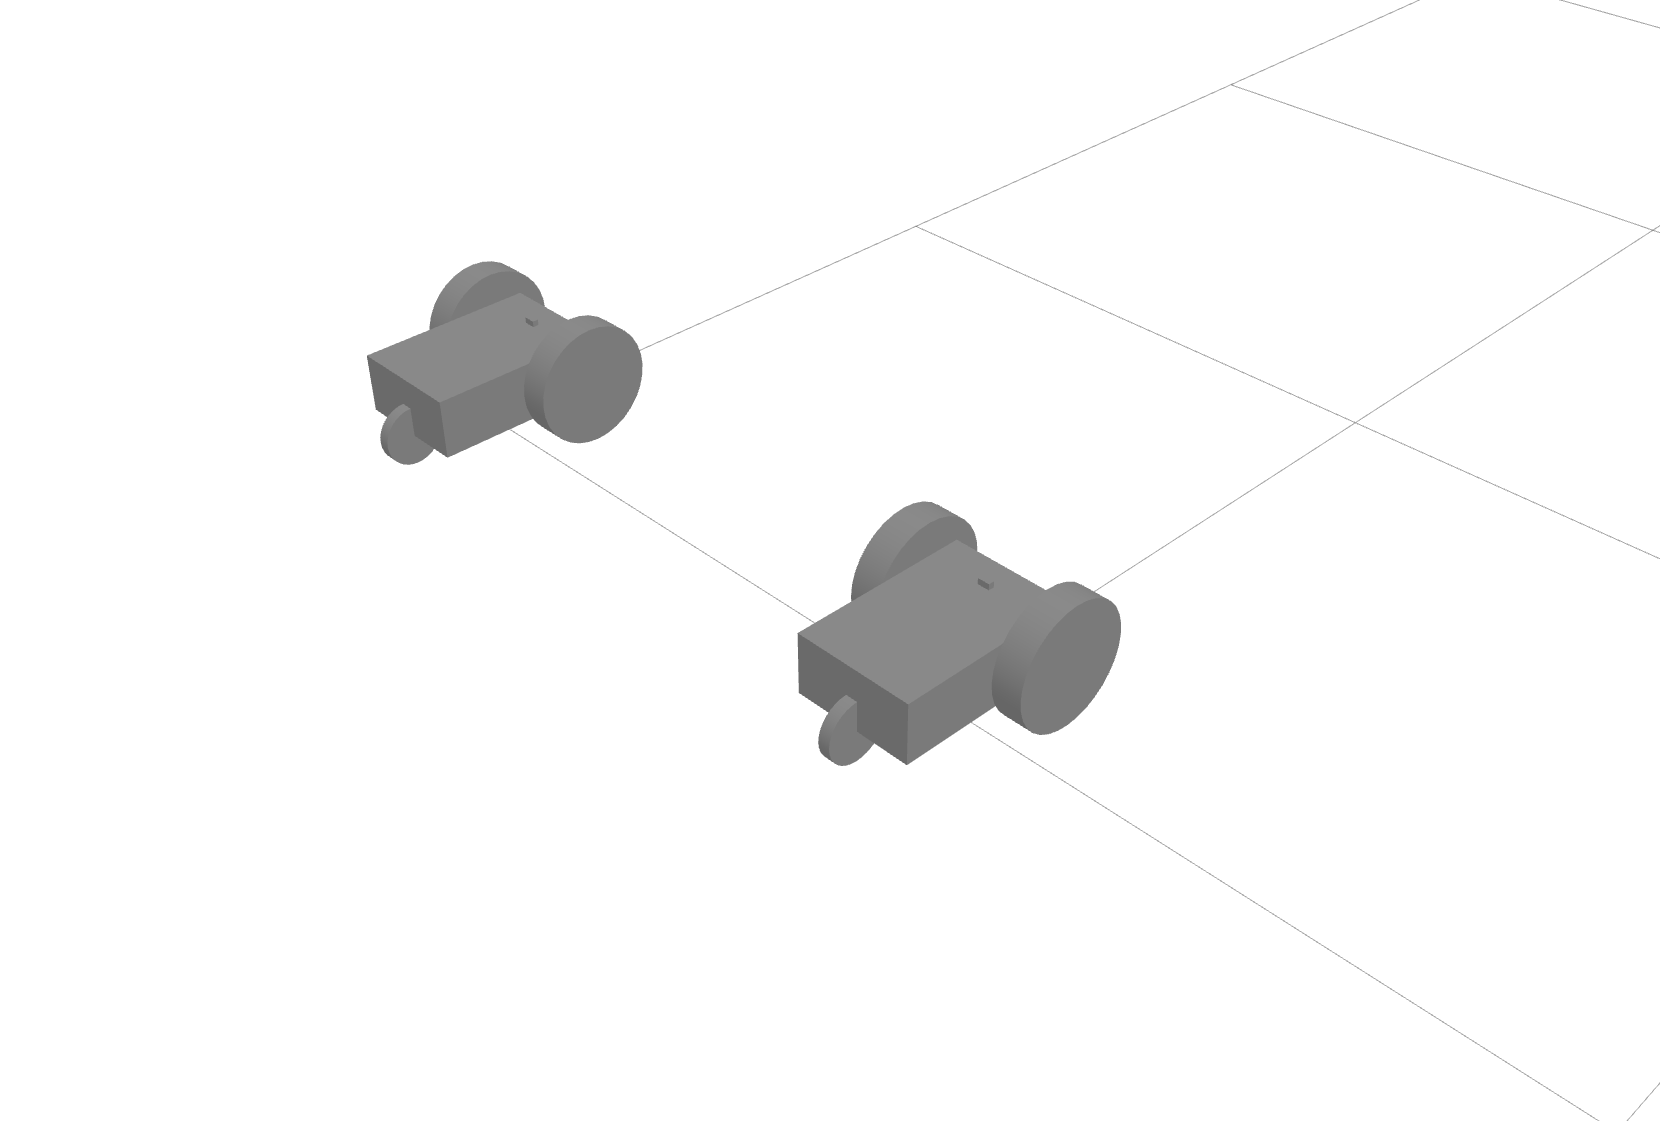
\includegraphics[width=0.5\textwidth]{graphics/crawlers.png}
	\caption{Crawler model used for acoustic inspection of metal structures.}
	\label{fig:crawler}
\end{figure}

Each robot is either a transmitter or a receiver, or both.
Crawlers are equipped with different sensors.
Among them :
\begin{itemize}
	\item an \gls{imu} sensor
	\item a piezoelectric or \gls{ugw} sensor
	\item a \gls{lidar} sensor
\end{itemize}
The \gls{imu} sensor makes it possible to know the orientation of the robot in the environment.
The \gls{ugw} sensor detects the presence of corrosion on the metal surface by emitting and receiving ultrasonic waves.
The \gls{lidar} sensor detects obstacles in the environment.
The obstacles considered here are mainly the various robots inspecting the metal surface.
Corrosion zones are detected by the emission of ultrasonic waves by a robot and the reception of these waves by another robot.
Insofar as the wave received by one of the crawlers is altered, then there is a point of corrosion between the transmitter robot and the receiver robot.
The detection of these corrosion zones is carried out in real time.
The maximum range of ultrasonic waves is noted $d_{max}$.
We approximate the propagation time of ultrasonic waves in the metal surface by zero time.

We use an occupancy grid to model the environment in which robots evolve during the acoustic inspection of metal structures.
This grid allows us to represent and categorize the different states of the areas of the metal surface.
The occupancy grid is composed of cells, where each cell corresponds to a small region of the environment.
In particular, we used a resolution of 0.05 meters per cell.
We use three states to characterize these cells: unknown, empty and occupied.
Unknown state refers to areas whose state has not yet been determined or detected.
The empty state indicates areas where there is no corrosion detected, i.e. the metal surface is sound.
Finally, the occupied state represents the identified corrosion areas, where the presence of defects or deterioration is detected.

By using this occupancy grid, we can track and update in real time the state of different areas of the metal surface during the inspection.
This allows us to plan robot movements, optimize their trajectory and ensure full coverage of the surface to be inspected.
In addition, this representation gives us a clear view of the state of corrosion of the metal structure, thus facilitating the analysis and evaluation of the results of the inspection.

In the rest of our proposal, we will detail the algorithms and methods used to update the occupancy grid according to the information collected by the robots' sensors.
We will also discuss multi-robot navigation strategies that leverage this modeling to optimize data acquisition and improve the efficiency of acoustic inspection.

\section{Background}

We present here the state of the art in the field of multi-robot navigation and control for the acoustic inspection of metal structures.
The objective of this literature review was to collect key information, analyze previous work and situate our project in the existing research context.
The references and sources cited in this section provide a solid foundation of knowledge and expertise on the subject.

Initially, we were interested in the properties of \gls{ugw}s and their applications in the field of tomography~\cite{OUABI2022106705, HUTHWAITE2013979}, mapping of robots and metallic structures~\cite{9364359, 9811581, inventions3030059, 9568841}, robots and sensors used in our project~\cite{s22093235}, multi-robot exploration~\cite{bautin:hal-00757960, articlesvsdf} as well as placement strategies for detection~\cite{article455556, 7487624, 7139673}.

In the paper~\cite{OUABI2022106705}, the authors propose a method to infer the geometry of metal plates using Lamb waves.
They use beamforming~\cite{enwiki:1151960654} to estimate plate boundaries based on acoustic measurements.
Experimental results show accurate inference of plate geometry.
However, the authors are content to map the contours of the structures, without proposing a method to map the defects, which is the subject of our problem.

The article~\cite{9364359} presents a FastSLAM-based approach~\cite{article254524} for robotic inspection of metal structures using ultrasound.
The authors propose a pioneer edge allocation method for multi-robot exploration, allowing fast and accurate inspection of structures.
Our work takes robot localization and mapping as known, and focuses on trajectory planning for the inspection of metal structures.
The approach used in this article can therefore be complementary to our work.

In the paper~\cite{9811581}, the authors propose a method for mapping metallic structures using \gls{ugw}s.
They combine a Cartesian grid with specific features for defect detection.
The experimental results show an accurate mapping of metallic structures.
However, the authors are once again content to map the outlines of the structures, without proposing a method for mapping the defects.

The article~\cite{inventions3030059} focuses on the localization of impacts in composite structures using a developed imaging method.
The authors use piezoelectric sensors~\cite{enwiki:1154129092} to detect and localize impacts, and a wavelet transform method~\cite{enwiki:1147185762} to analyze acoustic signals.
Experimental results show accurate detection and localization of impacts.
The sensors used are similar to those used in our project, but these sensors are positioned in a fixed way on the structure, while we want a mobile strategy.

In the paper~\cite{HUTHWAITE2013979}, the authors propose a high-resolution ultrasound tomography method for the quantification of wall thickness.
They exploit the dispersive nature of Lamb waves to convert variations in thickness into variations in wave velocity, thus enabling accurate reconstruction of wall thickness.
Experimental results show accurate reconstructions of corrosion defects.
This article was interesting to understand the properties of \gls{ugw}s and their applications in the field of tomography.

The article~\cite{s22093235}, resulting from the work of the BugWright2 project, presents a magnetic robot system for the inspection and autonomous maintenance of large structures.
The authors propose a localization framework based on a grid created from a point cloud, coupled with \gls{uwb} sensors and an \gls{imu}.
They also incorporate a piezoelectric sensor for \gls{ugw} detection for precise robot localization and structural feature mapping.
It is typically these robots and sensors that are used in our work.

The paper~\cite{bautin:hal-00757960} presents a planning algorithm for multi-robot exploration.
This algorithm, called \textit{MinPos}, is designed to efficiently allocate boundaries to robots in order to minimize the movement and time needed to explore the environment. It uses advanced optimization techniques to solve this problem effectively.
However, our work focuses on structural inspection for flaw detection.
We want a detailed inspection of corrosion areas and not a global exploration of the environment.

The article~\cite{article455556} presents strategies for the optimal placement of surveillance cameras in art galleries.
The authors propose methods to maximize surveillance coverage while minimizing the number of cameras needed.
However, the sensors used in our project are sensors that provide information on a segment only, between a transmitter and a receiver, and not global information like a camera.
The sensors used in our project are described in \ref{sec:definitions}.

In the article~\cite{articlesvsdf}, the authors propose a method for automatically locating and sizing defects in structures using guided wave imaging.
They use a convolutional neural network~\cite{enwiki:1159408824} to analyze guided wave signals and estimate defect sizes.
The experimental results show the efficiency of the proposed approach to invert both synthetic and experimental data.
This approach requires fixed sensors on the structure.
We want a mobile approach, not requiring the deployment of sensors on the structure.

The article~\cite{9568841} presents an autonomous on-plate exploration for an inspection robot using \gls{ugw}s.
The authors propose a localization method based on a mesh created from a cloud of points and use measurements from \gls{imu} and \gls{uwb} sensors.
They also integrate a piezoelectric sensor into the system for precise robot location and structural feature mapping.
In our approach, the location is assumed to be known.
This work can be used for robot localization, although this is not the subject of our project.
Nevertheless, the type of robot and sensors used are similar to those used in our project.

The article~\cite{7487624} presents effective measurement planning strategies for remote gas detection with mobile robots.
The objective of the study is to optimize the planning of measurements so as to maximize gas detection accuracy while minimizing the time and resources required.
The authors propose different approaches for planning measurements, including the use of exploration techniques based on the boundaries of detection zones, the selection of efficient trajectories to cover the environment and the reduction of the number of measurements necessary by using probabilistic models.
The type of sensor used has characteristics similar to those of the sensors used in our project.
However, our problem imposes movements of pairs of robots.
The way to split the investigation into two phases, a rough inspection phase and a refinement phase, is also similar to our approach.
However, this first phase is performed by fixed sensors, which is not desirable in our approach.
We will also use a \gls{tsp} to optimize robot movements between areas of interest.

In the paper~\cite{7139673}, the authors propose an efficient measurement planning method for remote gas detection with mobile robots.
Their approach is to optimize the planning of measures in order to minimize the time and resources required.
To do this, they use a convex relaxation technique in order to solve the optimization problem which allows to minimize the number of necessary measurements, while guaranteeing a complete coverage of the environment.
This study is interesting for our problem and could inspire improvements of our approach in the optimization of the \gls{tsp} used.

In summary, the works presented in this section are interesting for our problem, because they allowed us to deepen our knowledge of the problems related to guided wave tomography.
The articles~\cite{7487624, 7139673} are the closest to our problem.
However, these articles focus on covering the environment without worrying about the quality of the mapping of the areas of interest.
Moreover, these items use fixed sensors on the structure for the first rough inspection phase, which is not desirable in our approach.
This is why we propose a multi-robot navigation approach for the acoustic inspection of metallic structures in order to optimize the acquisition of data which will allow to carry out the tomography of metallic surfaces.


		
\chapter{Methodology}

\section{Solution Proposal}

We present our proposed solution for the acoustic inspection of metal structures using multi-robot navigation strategies.
We have developed three specific strategies to optimize data acquisition and enable the tomography of metallic surfaces.
These three strategies are:
\begin{enumerate}
	\item \textit{Roller Painting} navigation strategy
	\item \textit{Nordic Skiing} navigation strategy
	\item \textit{Polygonal Investigation} navigation strategy
\end{enumerate}
Among these strategies, the first two are non-reactive and can be considered as coarse exploration strategies, the goal being to quickly obtain a global coverage of the surface to be inspected.
The third strategy is reactive and makes it possible to optimize the acquisition of data for the realization of the tomography.
These three strategies aim to map the metal surface and detect areas of corrosion.
We define these three navigation strategies in the following subsections.
We also explain how the data structure used for mapping corrosion areas, an occupancy grid, is updated based on information collected by the robots' \gls{ugw} sensors.

\subsection{Occupancy Grid Update Process for Mapping}

When scanning the surface to be inspected by a pair of transmitter and receiver robots, the transmitter robot emits an acoustic wave in the metal structure, which is then received by the receiver robot.
The detection being considered as perfect, the receiver robot receives the wave emitted by the transmitter robot, without quasi-alteration of the power of the signal, if and only if the line segment between the two robots does not cross a zone of corrosion.
It is thus possible to determine whether a corrosion zone is present between the two robots by checking whether the signal received by the receiving robot is sufficiently powerful.
Insofar as there is no detection of corrosion between the transmitter and the receiver, then the line segment between the two robots is considered to be free of corrosion.
Otherwise, then the points of the line segment between the two robots are considered to be corrosion, with the exception of the points previously perceived to be free of corrosion.
The presence of corrosion on the segment is therefore overestimated.
The displacement strategies will aim to carry out several measurements, to reduce this overestimation, and approach the real shape of the corrosion.

We now only need to determine which cells of the occupancy grid are crossed by the line segment between the two robots.
For this we use Bresenham's segment drawing algorithm~\cite{enwiki:1155124335} which is commonly used to determine the points of a discrete plane that need to be drawn in order to form an approximation of a line segment between two given points.
We detail our implementation of this algorithm in \ref{subsec:Bresenham}.

As the metal surface is explored, the occupation grid is updated based on the information gathered by the robots.
More precisely, the cells of the occupancy grid that identify corrosion elements are updated with the occupied state, while the cells that identify healthy areas are updated with the empty state.
We thus end up with an occupation grid which represents the state of corrosion of the metal surface, with, for each corrosion zone, an approximation of the convex envelope of the corrosion zone.

\subsection{\textit{Roller Painting} Navigation Strategy}

The first navigation strategy we propose is the \textit{Roller Painting} navigation strategy.
We chose this name for this strategy because the movement of the robots during this strategy is similar to that of a paint roller when painting a wall.
This strategy is based on a rough exploration of the surface to be inspected, where the robots move in a straight line on parallel trajectories, guaranteeing global coverage of the inspection area.
It is therefore a question here of carrying out a grid of the surface to be inspected.

\begin{figure}[h!]
	\centering
	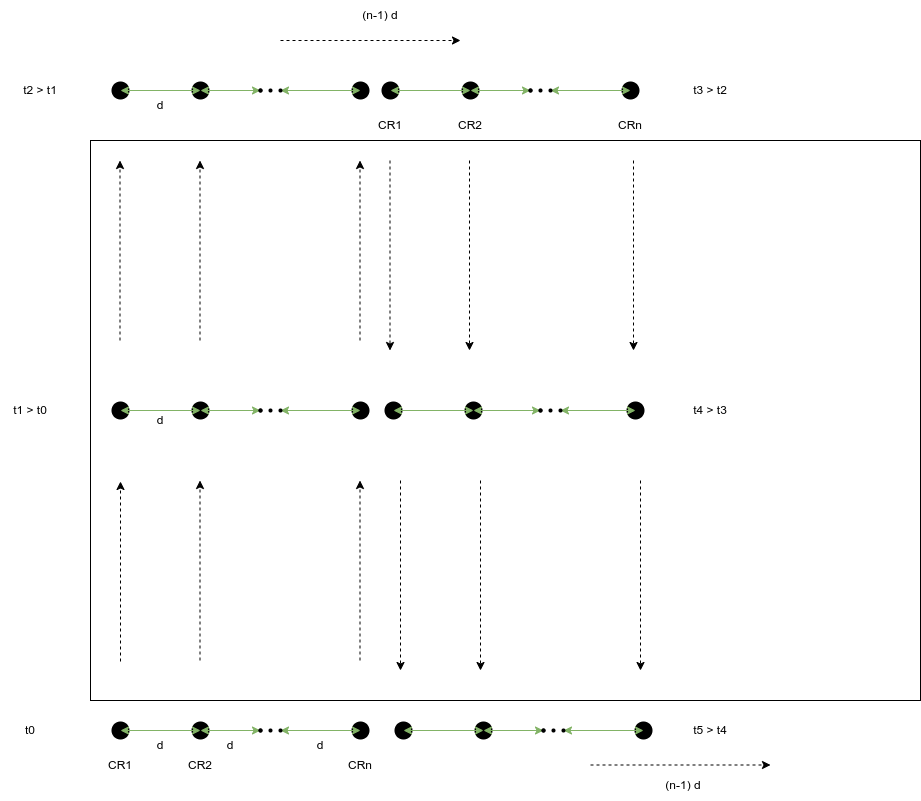
\includegraphics[scale=0.45]{graphics/peinture_au_rouleau.png}
	\caption{\textit{Roller Painting} navigation strategy - vertical phase.}
	\label{fig:peinture_au_rouleau}
\end{figure}

We present in \ref{fig:peinture_au_rouleau} a diagram describing the paint roller navigation strategy.
This strategy consists of two phases, a vertical movement phase and a horizontal movement phase.
The \ref{fig:peinture_au_rouleau} shows the first phase of vertical displacement.
In order to achieve this strategy, a minimum of $n \in \mathbb{N}$ robots, $n \ge 2$, aligned horizontally and separated by a distance $d < d_{max}$, is used.
These robots move vertically, simultaneously, following a parallel trajectory.
Once the end of the surface to be inspected has been reached, the robots rotate 90 degrees and move horizontally, simultaneously, by a distance $(n - 1) \cdot d$.
They then perform a new 90 degree rotation and move again vertically, in a straight line, simultaneously, following a path parallel to each other, until they reach the other end of the surface to be inspected.
This process is repeated until the metal surface is fully inspected.
The same process is then repeated, but this time horizontally.

During this strategy, each robot is both a transmitter and a receiver of \gls{ugw}s.
If the distance separating a robot $n_a$ from a robot $n_b$, $(n_a, n_b) \in \{1, 2, \dots, n\}^2$, is less than the maximum propagation distance of the \gls{ugw}s, $d_{max}$, then the robot $n_a$ is able to receive the signal emitted by the robot $n_b$ and vice versa.
However, it is not necessary for a robot $n_k$, $n_k \in \{1, 2, \dots, n\}$, to process signals received from all other robots.
Indeed, the robots being aligned, the signals received from the robots $n_{k-1}$ and $n_{k+1}$, are sufficient for the reconstruction of the state of the metallic surface.
The waves emitted by the robots $n_1, n_2, \dots, n_{k-2}$ and $n_{k+2}, \dots, n_n$ are not useful for the robot $n_k$.
The robot $n_k$ can therefore ignore these signals and concentrate only on the signals received from the robots $n_{k-1}$ and $n_{k+1}$.
Insofar as the first signals perceived by the robot $n_k$ are those emitted by the robots $n_{k-1}$ and $n_{k+1}$, due to their proximity, it is possible for the robot $n_k$ to filter signals received from other robots.
This constitutes an optimization in terms of processing for each robot.

The fact that the robots move along a parallel trajectory and simultaneously, implies that the rays of the signal emitted by the transmitter robot and received by the receiver robot, always have an orientation of $0$ radian for the vertical phase and an orientation of $\frac{\pi}{2}$ radians for the horizontal phase.
There is therefore not a large variation in the orientation of the transmitted and received signal.
Thus, this strategy will only be able to approach the convex envelopes of the corrosion zones by rectangles.
Examples of occupancy grids resulting from the \textit{Roller Painting} navigation strategy, represented as images, where the cells of the grid correspond to the pixels of the images, are shown in \ref{annexe:resultat}, \ref{fig:peinture_au_rouleau_resultats}.

\subsection{\textit{Nordic Skiing} Navigation Strategy}

The second strategy we propose is the navigation strategy \textit{Nordic Skiing}.
We chose this name for this strategy because the movement of the robots during this strategy is similar to the movement of a skier's skis.
This strategy still consists of moving in a straight line and following parallel trajectories, but this time the robots move sequentially and no longer simultaneously.
In this strategy, we wanted to increase the orientation diversity of the transmitted and received signal rays, in order to approach more precisely the convex envelopes of the corrosion zones.

\begin{figure}[h!]
	\centering
	\begin{subfigure}[t]{0.45\linewidth}
		\centering
		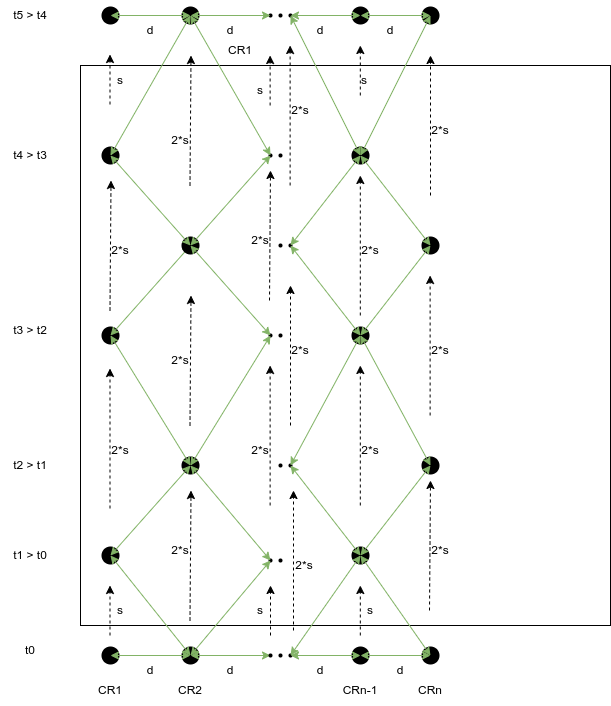
\includegraphics[width=\linewidth]{graphics/ski_nordique_1.png}
		\caption{\textit{Nordic Skiing} navigation strategy - first phase.}
		\label{fig:ski_nordique_1}
	\end{subfigure}
	\hfill
	\begin{subfigure}[t]{0.45\linewidth}
		\centering
		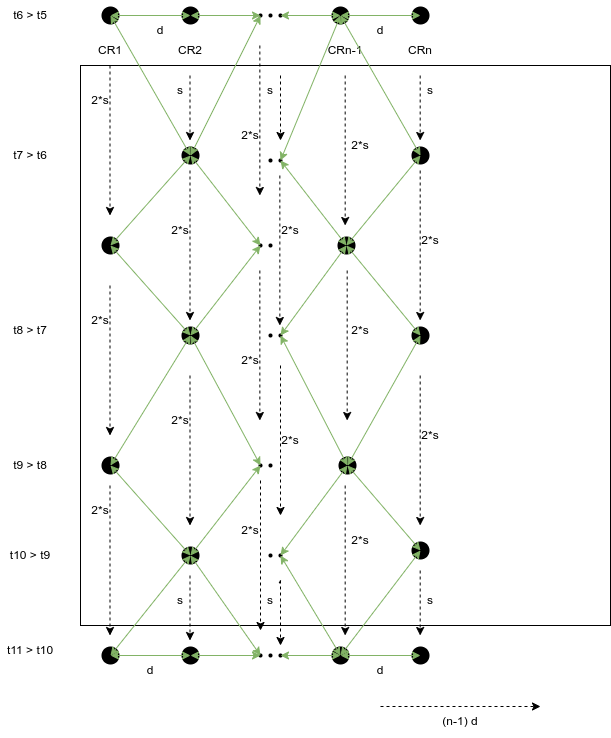
\includegraphics[width=\linewidth]{graphics/ski_nordique_2.png}
		\caption{\textit{Nordic Skiing} navigation strategy - second phase.}
		\label{fig:ski_nordique_2}
	\end{subfigure}
	\caption{\textit{Nordic Skiing} navigation strategy - vertical phase.}
	\label{fig:ski_nordique}
\end{figure}

\ref{fig:ski_nordique} presents a diagram describing the \textit{Nordic Skiing} navigation strategy.
This strategy also consists of two phases, a vertical movement phase and a horizontal movement phase.
\ref{fig:ski_nordique} shows the first phase of vertical movement.
In order to achieve this strategy, a minimum of $n \in \mathbb{N}$ robots, $n \ge 2$, aligned horizontally and separated by a distance $d < d_{max}$, is used.
These robots move vertically, following a parallel path, but sequentially.
The odd robots move in a straight line a distance $s$ and stop.
The even robots then move in a straight line a distance of $2 \cdot s$ and stop.
This process is repeated until the end of the surface is reached (\ref{fig:ski_nordique_1}).
Then, the robots repeat this same process, in the opposite direction and so that the stopping points of the robots are not the same as those previously (\ref{fig:ski_nordique_2}).
That is to say that this time, it is the even robots which start by moving in a straight line for a distance $s$ and then stop.
Then the odd robots move in a straight line for a distance of $2 \cdot s$ and then stop.
The robots then move horizontally a distance $(n - 1) \cdot d$ and repeat the same process until the metal surface is fully inspected.
The same process is then repeated, but this time horizontally.
In order for the various receiver robots to be able to receive the signals emitted by the transmitter robots, it is also necessary to impose that $s$ be strictly less than $\frac{d_{max}}{2}$, i.e. $s < \frac{d_ {max}}{2}$.

During this strategy, each robot is both a transmitter and a receiver of \gls{ugw}s.
Here, as with the \textit{Roller Painting} navigation strategy, it is not necessary for a robot $n_k$, $n_k \in \{1, 2, \dots, n\}$, to process the signals received by robots other than $n_{k-1}$ and $n_{k+1}$.

The fact that the robots move following a parallel trajectory, but in a sequential way, implies that the rays of the signal emitted by the transmitter robot and received by the receiver robot, have an orientation of greater variation.
Thus, this strategy makes it possible to approximate the convex envelopes of the corrosion zones by more diverse and precise shapes than rectangles.
Examples of occupation grids resulting from the \textit{Nordic Skiing} navigation strategy, represented in the form of images, where the cells of the grid correspond to the pixels of the images, are shown in \ref{annexe:resultat}, \ref{fig:ski_nordique_resultats} and \ref{fig:ski_nordique_resultats_2}.

\subsection{\textit{Polygonal Investigation} Navigation Strategy}

The third strategy we propose is the \textit{Polygonal Investigation} navigation strategy.
We have seen, previously, that at the end of the realization of the \textit{Roller Painting} navigation strategy, the convex envelope of the corrosion zones was approximated by a rectangle.
This approximation is a little more precise for the \textit{Nordic Skiing} navigation strategy.
It would be interesting to have a greater degree of precision around potential areas of corrosion.
This is what we propose with the \textit{Polygonal Investigation} navigation strategy.
This strategy consists of investigating around potential areas of corrosion, previously detected by one of the two previous navigation strategies.
It consists of positioning the robots around the corrosion zones and making them move along a polygonal trajectory, so that the rays of the signal emitted and received have an orientation of greater variation even around these zones.

\begin{figure}[h!]
	\centering
	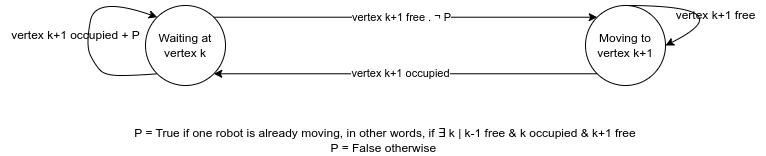
\includegraphics[scale=0.6]{graphics/automat_poly.png}
	\caption{\textit{Polygonal Investigation} navigation strategy.}
	\label{fig:automat}
\end{figure}

We present in \ref{fig:automat} a finite state automaton describing the \textit{Polygonal Investigation} navigation strategy.
At the beginning of the \textit{Polygonal Investigation} navigation strategy, each $n \in \mathbb{N}$ robots, $n \ge 2$, of $k \in \mathbb{N}$ teams, $k \ge 1$, are positioned on consecutive vertices of a polygon $P$ with $p \in \mathbb{N}$ vertices, $p \ge 3$, enclosing the potential area of corrosion.
To ensure the proper functioning of the strategy, it is necessary that the distance $d^*$, corresponding to the maximum distance between two vertices of the polygon $P$, be strictly less than $d_{max}$, i.e. $d^* < d_{max}$.
In the latter, each robot has two states.
The first consists of waiting and the second consists of moving along the polygonal trajectory, namely traversing the various vertices that make up the polygon.
The robot capable of advancing, that is to say, whose next vertex is not occupied by another robot, advances.
The others wait until the advancing robot reaches the last free vertex of the polygon.
The process is then repeated for each robot of each team until the vertices occupied by the robots are the same as those occupied at the beginning of the \textit{Polygonal Investigation} navigation strategy.

\begin{figure}[h!]
	\centering
	\begin{subfigure}[t]{0.27\linewidth}
		\centering
		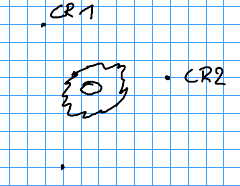
\includegraphics[width=\linewidth]{graphics/triangle_1.png}
		\caption{Initial phase, crawlers are positioned on consecutive vertices of the polygon.}
		\label{fig:triangle_1}
	\end{subfigure}
	\hfill
	\begin{subfigure}[t]{0.27\linewidth}
		\centering
		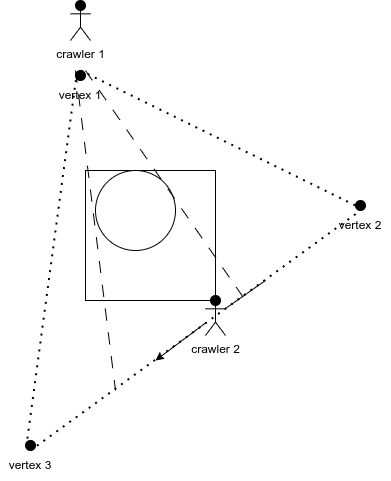
\includegraphics[width=\linewidth]{graphics/triangle_2.png}
		\caption{First phase of movement, crawler 2 moves from vertex 2 to vertex 3.}
		\label{fig:triangle_2}
	\end{subfigure}
	\hfill
	\begin{subfigure}[t]{0.27\linewidth}
		\centering
		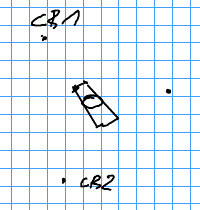
\includegraphics[width=\linewidth]{graphics/triangle_3.png}
		\caption{Second phase, crawler 2 reaches vertex 3 and stops.}
		\label{fig:triangle_3}
	\end{subfigure}
	\hfill
	\begin{subfigure}[t]{0.27\linewidth}
		\centering
		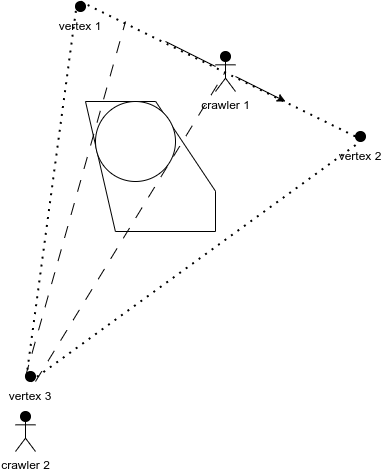
\includegraphics[width=\linewidth]{graphics/triangle_4.png}
		\caption{Second phase of movement, crawler 1 moves from vertex 1 to vertex 2.}
		\label{fig:triangle_4}
	\end{subfigure}
	\hfill
	\begin{subfigure}[t]{0.27\linewidth}
		\centering
		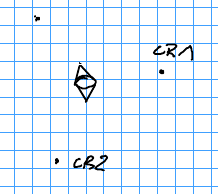
\includegraphics[width=\linewidth]{graphics/triangle_5.png}
		\caption{Third phase, crawler 1 reaches vertex 2 and stops.}
		\label{fig:triangle_5}
	\end{subfigure}
	\hfill
	\begin{subfigure}[t]{0.27\linewidth}
		\centering
		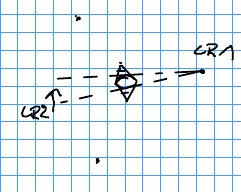
\includegraphics[width=\linewidth]{graphics/triangle_6.png}
		\caption{Third phase of movement, crawler 2 moves from vertex 3 to vertex 1.}
		\label{fig:triangle_6}
	\end{subfigure}
	\hfill
	\begin{subfigure}[t]{0.27\linewidth}
		\centering
		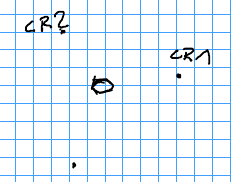
\includegraphics[width=\linewidth]{graphics/triangle_7.png}
		\caption{Last phase, crawler 2 reaches vertex 1 and stops.}
		\label{fig:triangle_7}
	\end{subfigure}
		\caption{Movement phases of the \textit{Polygonal Investigation} navigation strategy.}
		\label{fig:triangle}
\end{figure}

We present in \ref{fig:triangle} an example of the different moving phases of the \textit{Polygonal Investigation} navigation strategy with $k = 1$ team, $n = 2$ robots and $p = 3$ vertices.
On these different figures, we have represented a corrosion zone by a circle and an approximation of this zone by a square enveloping the circle, as we can see in \ref{fig:triangle_1}.
The objective is to approach the corrosion zone as finely as possible.
The corrosion zone is not known in advance, only the shape of the square enveloping the circle is known.
\ref{fig:triangle_1} presents the initial phase of the \textit{Polygonal Investigation} navigation strategy, where the two crawlers are positioned on consecutive vertices of the polygon.
\ref{fig:triangle_2} shows the first moving phase of the \textit{Polygonal Investigation} navigation strategy, while the crawler 2 moves from vertex 2 to vertex 3, until it reaches the latter, as we can see in \ref{fig:triangle_3}.
We can see that after the crawler 2 has reached vertex 3, part of the suspected corrosion area is removed and considered healthy, as we can see in \ref{fig:triangle_3}.
The crawlers keep moving until they reach their initial position, as we can see in \ref{fig:triangle_7}.

\begin{definition}[Phantom zone]
	\label{def:fantomas}
	A phantom zone is a corrosion zone detected by one of the navigation strategies, but which is not a corrosion zone. It is a false positive.
\end{definition}

The \textit{Polygonal Investigation} navigation strategy has two advantages.
The first is that it quickly eliminates phantom zones (\ref{def:fantomas}).
The second is that it makes it possible to approach the convex envelopes of the corrosion zones by more diverse and precise shapes than rectangles due to the great variation in the orientation of the rays of the signal emitted and received by the robots around each vertex of the polygon.

This strategy requires two steps prior to its execution:
\begin{enumerate}
	\item the extraction of the corrosion zones detected by one of the preceding navigation strategies.
	\item determining the order of investigation of corrosion areas.
\end{enumerate}

The first step can be solved using a \gls{scc} graph decomposition algorithm.
A \gls{scc} is defined in \ref{def:scc}.
We then consider our occupation grid, resulting from the exploration of one of the two previously defined strategies, as an undirected graph $G = (V, E)$, where $V$ is the set of vertices of the graph, corresponding to the cells of the occupancy grid and $E$ is the set of edges of the graph, corresponding to the adjacent cells of the occupancy grid.
This problem is well known and there are simple algorithms to solve it, such as Tarjan's algorithm~\cite{enwiki:1148118528}, of linear time complexity $O(|V| + |E|)$.
We will not look further into this problem and entrust its resolution to the \textit{OpenCV} library.

\begin{definition}[\gls{scc}]
	\label{def:scc}
	A strongly connected component of a graph $G = (V, E)$ is a subset $C$ of $V$ such that for any pair of vertices $(u, v) \in C^2$, there is a path from $u$ to $v$ and a path from $v$ to $u$.
\end{definition}

\begin{definition}[Hamiltonian cycle]
	\label{def:hamilton}
	A Hamiltonian cycle is a cycle passing through all the vertices of a graph, once and only once.
\end{definition}

\begin{definition}[\gls{tsp}]
	\label{def:tsp}
	Given a graph $G = (V, E)$, where $V$ is the set of vertices of the graph and $E$ is the set of edges of the graph, and a cost function $c : E \rightarrow \mathbb{R}$, the \gls{tsp} consists in finding a Hamiltonian cycle (\ref{def:hamilton}) of minimal cost in $G$.
\end{definition}

\begin{definition}[Multi-depot \gls{mtsp}]
	\label{def:mtsp}
	Given a graph $G = (V, E)$, where $V$ is the set of vertices of the graph and $E$ is the set of edges of the graph, a cost function $c : E \rightarrow \mathbb{R}$, and a set of depots $D \subset V$, the multi-depot \gls{mtsp} is to find a set of cycles of minimum total cost in $G$, each going through one and only one deposit.
\end{definition}

The second step can be solved using a \gls{tsp} (\ref{def:tsp}) algorithm in the case where the number of teams $k$ is equal to 1 and a \gls{mtsp} (\ref{def:mtsp}) algorithm in the case where the number of teams $k$ is strictly greater than 1.
There are several solution paradigms to solve this type of problem.
A first is to find an exact solution using an integer linear programming algorithm.
A second is to find an approximate solution using a meta-heuristic.

\begin{definition}[\gls{np} Class]
	\label{def:np}
	The class \gls{np} is the class of decision problems that can be solved by a non-deterministic algorithm in polynomial time.
\end{definition}

\begin{definition}[\gls{np}-hard problem]
	\label{def:nph}
	A problem is \gls{np}-hard if it is at least as hard as problems of class \gls{np}.
	In other words, a problem is \gls{np}-hard if there is a polynomial reduction algorithm that transforms a problem of class \gls{np} into an instance of this problem.
\end{definition}

\begin{definition}[\gls{np}-complete problem]
	\label{def:npc}
	A problem is \gls{np}-complete if it is both \gls{np} and \gls{np}-hard.
\end{definition}

The \gls{tsp} is a \gls{np}-complete (\ref{def:npc}) problem.
It can be treated as an integer linear optimization problem~\cite{article244, gurobi25}.
To do this, we use the formulation presented in \ref{eq:tsp}.

\begin{equation}
	\label{eq:tsp}
	\begin{array}{ll@{}rr}
		\text{minimize} &
		\displaystyle\sum\limits_{i \in V} \sum\limits_{j \in V} c_{ij} x_{ij} &
		&
		\\
		\text{subject to} &
		\displaystyle\sum\limits_{i \in V} x_{ij} = 1 &
		&
		\forall j \in V \\
		&
		\displaystyle\sum\limits_{j \in V} x_{ij} = 1 &
		&
		\forall i \in V \\
		&
		\displaystyle\sum\limits_{i \in S} \sum\limits_{j \in S} x_{ij} \leq |S| - 1 &
		&
		\forall S \subset V, 2 \leq |S| \leq |V| - 1 \\
		&
		x_{ij} \in \{0, 1\} &
		&
		\forall i \in V, \forall j \in V \\
	\end{array}
\end{equation}

The objective function to be minimized from the \ref{eq:tsp} is the sum of the distances between each pair of locations.
The first two constraints ensure that each city is visited exactly once.
The third constraint ensures that the cycle formed by the cities visited is simple, that is to say, that it does not contain sub-cycles.
The last constraint ensures that the decision variables $x_{ij}$ are binary, with $x_{ij} = 1$ if the robot moves from city $i$ to city $j$ and $x_{ij} = 0$ otherwise.

The \gls{mtsp} is an \gls{np}-hard problem (\ref{def:nph})~\cite{SUNDAR201639}.
This one can be solved using meta-heuristics like a genetic algorithm~\cite{SinghMTSP, Kiraly2011}

In the next sections, we will detail each navigation strategy, exposing the specific algorithms and mechanisms used to implement our proposed solution. We will also analyze the performance and results obtained through extensive experimentation and evaluation.

\section{Algorithm Implementations}

In this section, we highlight some of the different technical implementations we have developed to support our multi-robot navigation and control solutions in the context of acoustic inspection of metal structures.
We begin by describing our adaptation of Bresenham's line algorithm~\cite{enwiki:1155124335}, widely used to determine which points of a discrete plane should be plotted in order to form a segment approximation of line between two given points.
Next, we discuss the implementation of the \textit{Roller Painting} algorithm, which allows the robots to move simultaneously, following parallel trajectories.
We continue with the implementation of the \textit{Nordic Skiing} algorithm, which allows the robots to move alternately, following parallel trajectories, thus modifying the orientation of the vector representing the direction of movement of the wave transmitted and received by the pair of robots.
Additionally, we look at the implementation of the \textit{Polygonal Investigation} algorithm, which allows robots to examine suspected areas of corrosion more precisely.
Finally, we present Cohen's $\kappa$ algorithm~\cite{enwiki:1130024730}, used to assess the quality and reliability of the acoustic inspection results.
We discuss in detail our implementation of this algorithm, which provides quantitative measures to evaluate the performance of robots in the inspection of metal structures.
Each of these technical implementations contributes to the efficiency and accuracy of our multi-robot navigation and control approach, and will be discussed in detail in the following subsections.

\subsection*{Bresenham's Line Algorithm}\label{subsec:Bresenham}

\begin{algorithm}[h!]
	\caption{Process of updating the occupancy grid using Bresenham's line algorithm.}
	\label{alg:Bresenham}
	\KwData{$P_1 \in \mathbb{R}^2$, $P_2 \in \mathbb{R}^2$, $pw \in \mathbb{R}$, $threshold \in \mathbb{R}$, $G$: $l \times w \rightarrow [\text{UNKNOWN}, \text{EMPTY}, \text{OCCUPIED}]$, $l \in \mathbb{N}$, $w \in \mathbb{N}$ \\
		with $P_1$ and $P_2$ the two points to connect, $pw$ the power of the \gls{ugw}, $threshold$ the threshold above which the power of the \gls{ugw} is considered undistributed and $G$ the grid to update.}
	\KwResult{The updated grid.}
	$p_0 \gets \text{from\_position\_to\_grid\_coordinate}(P_1)$ \\
	$p_1 \gets \text{from\_position\_to\_grid\_coordinate}(P_2)$ \\
	\If{\text{is\_out\_of\_grid}($p_0$) \textbf{or} \text{is\_out\_of\_grid}($p_1$)}{
		\Return
	}
	$dx \gets p_1.x - p_0.x$ \\
	$dy \gets p_1.y - p_0.y$ \\
	$sx \gets \text{sign}(dx)$ \\
	$sy \gets \text{sign}(dy)$ \\
	$err = dx - dy$ \\
	\While{$p_0 \neq p_1$}{
		\If{$pwd \leq threshold$ \textbf{and} $G(p_0) = \text{UNKNOWN}$}{
			$G(p_0) \gets \text{OCCUPIED}$
		}
		\ElseIf{$pwd > threshold$}{
			$G(p_0) \gets \text{EMPTY}$
		}
		$e2 \gets 2 \times err$ \\
		\If{$e2 > -dy$}{
			$err \gets err - dy$ \\
			$p_0.x \gets p_0.x + sx$
		}
		\If{$e2 < dx$}{
			$err \gets err + dx$ \\
			$p_0.y \gets p_0.y + sy$
		}
	}
\end{algorithm}

We use Bresenham's line algorithm to determine the points of the line segment between the two robots.
The algorithm is presented in \ref{alg:Bresenham}.
The part adapted to our problem is between lines 12 and 17 of the latter.
At this point, we check if the signal strength is sufficiently impaired and if the point of the line segment between the two robots has not already been perceived as free of corrosion.
If so, then the considered point is marked as corrosion, modeled by the value \texttt{OCCUPIED}.
If the signal strength is not sufficiently altered, then the considered point is marked as being free of corrosion, modeled by the value \texttt{EMPTY}.
Once all the points of the segment have been traversed, the grid $G$ is updated with the new information.
Bresenham's line algorithm thus contributes to the construction of the occupation grid which makes it possible to locate the corrosion zones detected by the robots during the acoustic inspection of metal structures.

\subsection*{\textit{Roller Painting} and \textit{Nordic Skiing} Algorithms}

We present in this subsection the implementations of the \textit{Roller Painting} and \textit{Nordic Skiing} algorithms.
Their source code is available on GitLab, here\footnote{\url{https://gitlab.georgiatech-metz.fr/bugwright2/bugwright2-ws/blob/cr_nav_strat/bugwright_ws/src/floor_nav/missions/peinture_au_rouleau.py}} and here\footnote{\url{https://gitlab.georgiatech-metz.fr/bugwright2/bugwright2-ws/blob/cr_nav_strat/bugwright_ws/src/floor_nav/missions/ski_nordique.py}}.

The implementations of these algorithms have been made using the Python programming language and the \gls{ros} libraries.
In these implementations, we use the \gls{ros} Task Manager~\cite{ROSTaskManager} framework to manage the tasks of the robot inspectors.
First, we initialize the \gls{ros} node and create a task client.
Then, we retrieve the necessary parameters such as the speed of the crawlers, the crawler identifier, the distance between the crawlers, the overlap or the dimensions of the surface to be inspected.

The algorithms are then executed following a sequence of precise movements.
For each crawler, we define vertical and horizontal trajectories using an iterative loop and mathematical calculations.
Crawlers move along defined paths, using task client functions such as \texttt{AlignWithTarget} and \texttt{FollowLine} to maintain a precise path.

During the execution of the algorithms, the crawlers synchronize using the \texttt{SetStatusSync} and \texttt{WaitForStatusSync} functions of the task client.
This ensures that the crawlers perform the movements in a coordinated manner and position themselves correctly to cover the entire metal surface.
At the end of each movement step, the status is updated and synchronization is performed with the corresponding partner.

The implementation of the two algorithms \textit{Roller Painting} and \textit{Nordic Skiing} allow crawlers to explore the metal surface in a methodical and complete way.
Using vertical and horizontal trajectories, crawlers traverse the surface overlapping previously inspected areas to ensure optimal coverage.
Here we have used a 10 cm overlap between the different vertical and horizontal trajectories.

Once the algorithms are completed, the execution time is recorded, providing an indication of how long it took to inspect the metal surface.
The occupancy grid is also recorded in order to calculate the inspection score.
This implementation is an essential step in our proposed solution for the acoustic inspection of metal structures and guarantees complete and effective coverage of the surface to be inspected.

\subsection*{\textit{Polygonal Investigation} Algorithm}

We present in this subsection the implementation of the \textit{Polygonal Investigation} algorithm.
The corresponding source code is available on GitLab~\footnote{\url{https://gitlab.georgiatech-metz.fr/bugwright2/bugwright2-ws/blob/cr_nav_strat/bugwright_ws/src/floor_nav/missions/investigation_polygonale.py}} .

The implementation of this algorithm was also carried out using the Python programming language and the \gls{ros} libraries.
In this implementation, we still use the \gls{ros} Task Manager~\cite{ROSTaskManager} framework to manage the tasks of the inspector robots.
First, we initialize the \gls{ros} node and retrieve the different parameters and more particularly the map of potential corrosion zones, on which we base ourselves for the inspection, which come from one of the two coarse strategies.
Next, we extract the \gls{scc} from the map using the \texttt{connectedComponentsWithStats} function from the \textit{OpenCV} library.
This function uses Bolleli's spaghetti algorithm~\cite{BolelliSpaghetti} to extract \gls{scc} from an image.
For each of these components, we retrieve its center and its dimensions.
Next, we construct a $p \in \mathbb{N}$ sided polygon around each center of a component.
To do this, we place $p$ points on an ellipse centered on the center of the component and whose axes are the dimensions of the component.
We therefore have for each potential zone of corrosion a polygon with $p$ sides which surrounds it.
All that remains is to find the shortest path that passes through all the polygons.
For this, we use the \textit{Gurobi} library to solve a simple \gls{tsp} in the case where the number of teams of robots $k = 1$.
When $k > 1$, we use the genetic algorithm proposed by Elad Kivelevitch~\cite{MDMTSPV_GA} to solve the multi-depot \gls{mtsp}.

Once the algorithms are completed, the run time is recorded, providing an indication of how long it will take to inspect the various potential areas of corrosion.
The occupancy grid is also recorded in order to calculate the inspection score.
This implementation is an essential step in our proposed solution for the acoustic inspection of metal structures and allows us to investigate potential areas of corrosion in an efficient way.

\subsection*{Algorithm for Calculating Cohen's $\kappa$}

Assessing the quality and reliability of acoustic inspection results is essential to ensure accurate measurements of the condition of metal structures.
In this subsection, we present the algorithm for calculating Cohen's $\kappa$~\cite{enwiki:1130024730}, introduced in \ref{alg:Cohen_Kappa}, a statistical measure commonly used to assess the agreement between the results obtained by the robots and a human reference.

\begin{table}[h!]
	\centering
	\begin{tabular}{|c|c|}
		\hline
		$\kappa$ & Interpretation \\
		\hline
		$< 0$ & Disagreement \\
		\hline
		$0.00 - $0.20 & Very Low agreement \\
		\hline
		$0.21 - $0.40 & Low agreement \\
		\hline
		$0.41 - $0.60 & Moderate agreement \\
		\hline
		$0.61 - $0.80 & Strong agreement \\
		\hline
		$0.81 - $1.00 & Almost perfect agreement \\
		\hline
	\end{tabular}
	\caption{Interpretation of Cohen's $\kappa$ according to Landis and Koch.}
	\label{tab:Kappa_Cohen}
\end{table}

Cohen's $\kappa$ calculation algorithm is based on the notion of concordance and discordance between the results of inspections carried out by robots and those carried out by human inspectors (ground truth).
It takes into account the positive, negative, false positive and false negative results obtained during the acoustic inspection.
This information is used to calculate the value of the Cohen coefficient, noted $\kappa$, with $\kappa = \frac{p_o - p_e}{1 - p_e}$, where $p_o$ is the observed rate of agreement and $p_e$ the expected agreement rate.

\begin{algorithm}[h!]
	\caption{Cohen's $\kappa$ algorithm.}
	\label{alg:Cohen_Kappa}
	\KwData{$I_0$: $l \times w \times 3 \rightarrow [0 .. 255]$, $I$: $l \times w \times 3 \rightarrow [0 .. 255]$, $l \in \mathbb{N}$, $w \in \mathbb{N}$ \\
		with $I_0$ the ground truth image and $I$ the image to score.}
	\KwResult{$\kappa \in [0, 1]$}
	$TP \gets 0$ \\
	$TN \gets 0$ \\
	$FP \gets 0$ \\
	$FN \gets 0$ \\
	\For{$i \gets 1$ \KwTo $l$}{
		\For{$j \gets 1$ \KwTo $w$}{
			\If{$\text{is\_label\_1}(I_0(i, j))$}{
				\If{$\text{is\_label\_1}(I(i, j))$}{
					$TP \gets TP + 1$
				}
				\Else{
					$FN \gets FN + 1$
				}
			}
			\Else{
				\If{$\text{is\_label\_1}(I(i, j))$}{
					$FP \gets FP + 1$
				}
				\Else{
					$TN \gets TN + 1$
				}
			}
		}
	}
	$f_c \gets \frac{(TN + FN) (TN + FP) + (FP + TP) (FN + TP)}{TP + TN + FN +FP}$ \\
	$\kappa \gets \frac{TP + TN - f_c}{TP + TN + FN + FP - f_c}$
\end{algorithm}

The algorithm proceeds in several steps.
First, the results of the inspections carried out by the robots and the actual distributions of the corrosion zones are compared for each zone inspected.
To do this, we compare the values of each cell of the occupancy grid, obtained at the end of the inspection by the robots, with those of the ground truth.
Having modeled the different test environments, we know the true distribution of the corrosion zones.
Then, the results are grouped into four categories: positive agreement, negative agreement, positive discrepancy (false positives), and negative discrepancy (false negatives).
These categories are used to calculate the observation and agreement rates observed between the robots and the true distribution of the corrosion zones.
Cohen's $\kappa$ is then calculated from observed observation and agreement rates, taking into account the possibility of concordance due to chance.
The closer Cohen's $\kappa$ is to 1, the greater the agreement between the robot results and the ground truth results.
On the other hand, a $\kappa$ close to 0 indicates a low level of agreement, while a negative $\kappa$ suggests a discrepancy between the results.
An interpretation of Cohen's $\kappa$ according to Landis and Koch is presented in \ref{tab:Kappa_Cohen}.

We implemented this algorithm in our project, using the results of the acoustic inspections carried out by the robots and the maps composed of corrosion zones as a basis for comparison.
This implementation allows us to obtain quantitative measures to evaluate the performance of our multi-robot navigation and control approach in the inspection of metal structures.
In the next sections, we will detail the results obtained thanks to the application of this algorithm of the calculation of Cohen's $\kappa$.

\section{Experiments}

In this section, we present the experiments we conducted to validate and evaluate our different multi-robot navigation and control strategies in the context of acoustic inspection of metal structures.
These experiments aim to demonstrate the efficiency, precision and reliability of our system in detecting and locating corrosion zones.

To carry out these steps, we chose to perform our experiments using \textit{Gazebo}, a well-established simulation environment in the field of robotics.
We started by building several test maps.
These maps model a flat surface on which are placed simple geometric shapes, rectangles and circles, and more complex shapes, polygons between 3 and 8 vertices.
These different geometric shapes represent the corrosion areas that we want to detect and locate.
We present in \ref{annexe:cartes}, in \ref{fig:test_models} the maps we built for our experiments.
Each of these cards is sized 6 meters by 6 meters.
The number of corrosion zones varies between 5, 8, 11, 15, 20 and 30 zones.
The size and location of corrosion areas are randomly generated.
For the maps of 5, 8, 11 and 15 zones, we generated 5 different maps in order to have more representative results.
We did not allow ourselves to generate several maps for the 20 and 30 zone maps, the polygonal investigation time being too long.

We also simulated the \gls{ugw} sensor by exploiting the simulation of a \gls{uwb} sensor.
This \gls{uwb} sensor makes it possible to emit a pulse and to receive it.
By measuring the signal strength, we are able to know whether the signal has passed through an object or not.
The behavior of this \gls{uwb} sensor is therefore similar to that of the \gls{ugw} sensor, namely that it makes it possible to detect the presence of an object between two points, but not to locate it.

We evaluated the performance of the three navigation strategies in terms of Cohen's $\kappa$ and inspection time.
For the \textit{Roller Painting} and \textit{Nordic Skiing} strategy, we only used two robots.
For these two strategies, we varied the distance $d$ between the robots.
For the \textit{Nordic Skiing} strategy, we also varied the stride $s$ between the robots.
For the \textit{Polygonal Investigation} strategy, we vary the number of robots $n$, the number of teams $k$ and the number of sides $p$ of the polygons used.
We use the result of the \textit{Roller Painting} navigation strategy as a starting point for the \textit{Polygonal Investigation} strategy.
We justify this choice by the fact that this strategy is the fastest and least accurate and therefore the most likely to benefit from an improvement from the \textit{Polygonal Investigation} strategy, without reaching inspection times too long.
We therefore vary the parameter $d$ of this strategy.
We summarize the experimental parameters used for each strategy in \ref{tab:exp_params}.

\begin{table}[h!]
	\centering
	\begin{tabular}{|c|c|c|}
		\hline
		Strategy & Parameter & Values \\
		\hline
		\multirow{2}{*}{\textit{Roller Painting}} & $n$ & 2 \\
		& $d$ & 1, 2, 3, 6 (meters) \\
		\hline
		\multirow{3}{*}{\textit{Nordic Skiing}} & $n$ & 2 \\
		& $d$ & 1, 2, 3, 6 (meters) \\
		& $s$ & 1, 2, 3, 6 (meters) \\
		\hline
		\multirow{5}{*}{\textit{Polygon Investigation}} & initial strategy & \textit{Roller Painting} \\
		& $d$ & 1, 2, 3, 6 (meters) \\
		& $n$ & 2 \\
		& $k$ & 1 \\
		& $p$ & 4, 6 \\
		\hline
	\end{tabular}
	\caption{Experimental settings used for each navigation strategy.}
	\label{tab:exp_params}
\end{table}

During these simulations, we expect to have certain results.
Among them, we expect the \textit{Roller Painting} strategy to be the fastest, but also the least accurate.
Conversely, we expect the \textit{Polygonal Investigation} strategy to be the most accurate, but also the slowest.
We also expect the $d$ parameter to have an impact on the accuracy and inspection time of the \textit{Roller Painting} and \textit{Nordic Skiing} strategies.
A low $d$ distance should provide better accuracy, but should also increase inspection time.
Moreover, we expect that the $s$ parameter will also have an impact on the accuracy and inspection time of the \textit{Nordic Skiing} strategy.
A low $s$ stride should provide better accuracy, but should also increase inspection time.
We also expect the $p$ parameter to have an impact on the accuracy and inspection time of the \textit{Polygonal Investigation} strategy.
A low number of sides $p$ should provide better accuracy, but should also increase inspection time.
Next, we expect the parameters $k$ and $n$ to have an impact on the inspection time of the \textit{Polygonal Investigation} strategy.
A high number of teams $k$ or a high number of robots $n$ should allow to obtain a lower inspection time.
Finally, we expect the number of corrosion zones to have an impact on the inspection time of the \textit{Polygonal Investigation} strategy, but not on the \textit{Roller Painting} and \textit{Nordic Skiing} strategies.
The higher the number of corrosion areas, the higher the inspection time should be for the \textit{Polygonal Investigation} strategy.
Finally, we expect the number of corrosion zones to have an impact on the accuracy of the different strategies.
The greater the number of corrosion areas, the lower the accuracy should be.
Indeed, the higher the number of corrosion zones, the higher the probability of phantom zones appearing for the \textit{Roller Painting} and \textit{Nordic Skiing} strategies.
For the \textit{Polygonal Investigation} strategy, the higher the number of corrosion zones, the greater the probability that two distinct corrosion zones were confused into one during the \textit{Roller Painting} or \textit{Nordic Skiing} strategies.

% \begin{table}[h!]
% 	\centering
% 	\begin{tabular}{|c|c|c|c|}
% 		\hline
% 		Strategy & Parameters & Score & Time \\
% 		\hline
% 		\multirow{5}{*}{\textit{Roller Painting}} & medium density, $d$ medium & - & ++ \\
% 		\cline{2-4}
% 		& low density & + & ++ \\
% 		& high density & - - & ++ \\
% 		& low $d$ & + & + \\
% 		& strong $d$ & - - & +++ \\
% 		\hline
% 		\multirow{7}{*}{\textit{Nordic Skiing}} & medium density, $d$ medium, $s$ medium & ++ & - \\
% 		\cline{2-4}
% 		& low density & +++ & - \\
% 		& high density & + & - \\
% 		& low $d$ & +++ & - - \\
% 		& strong $d$ & + & + \\
% 		& low $s$ & +++ & - - \\
% 		& strong $s$ & + & + \\
% 		\hline
% 		\multirow{9}{*}{\textit{Polygonal Investigation}} & mean density, mean $n$, mean $k$, mean $p$ & +++ & - \\
% 		\cline{2-4}
% 		& low density & ++++ & + \\
% 		& high density & ++ & - - \\
% 		& low $n$ & +++ & - - \\
% 		& strong $n$ & +++ & + \\
% 		& low $k$ & +++ & - - \\
% 		& loud $k$ & +++ & + \\
% 		& low $p$ & ++ & + \\
% 		& strong $p$ & ++++ & - - \\
% 		\hline
% 	\end{tabular}
% 	\caption{Expected results for each navigation strategy.}
% 	\label{tab:expected_results}
% \end{table}

% For the sake of clarity, we summarize in table~\ref{tab:expected_results} the expected results for each navigation strategy.
% The table presents the expected results for each navigation strategy, according to the different experimental parameters.
% Navigation strategies include \textit{Roller Painting}, \textit{Nordic Skiing}, and \textit{Polygonal Investigation}.
% Parameters include density, distance $d$, pitch $s$, number of sides of a polygon used in polygonal investigation $p$, number of teams $k$ and number of robots $ n$.

% For each strategy, the table indicates the expected scores and times associated with each of the parameters compared to the expected scores and times for the intermediate parameters.
% The scores are represented by "+" and "-" symbols and indicate the expected level of precision.
% The times are also indicated by "+" and "-" symbols and reflect the expected inspection slowness.
% Thus a ++ score is considered more accurate than a + score, and a - - time is considered slower than a - time, for example.

The different results from the different simulations carried out are available in \ref{annexe:resultat}.
On these images, it is possible to see in black the real areas of corrosion and in blue the areas detected as having corrosion by the various navigation algorithms.


		
\chapter{Results}

\subsection*{\textit{Roller Painting} navigation strategy}

We summarize in figure~\ref{fig:peinture_au_rouleau-kappa_vs_world} the evolution of the Cohen score as a function of the density of the world for each value of $d$.
We also summarize in figure~\ref{fig:peinture_au_rouleau-time_vs_world} the evolution of the inspection time according to the density of the world for each value of $d$.

\begin{figure}[h!]
	\centering
	\begin{subfigure}[t]{0.9\linewidth}
		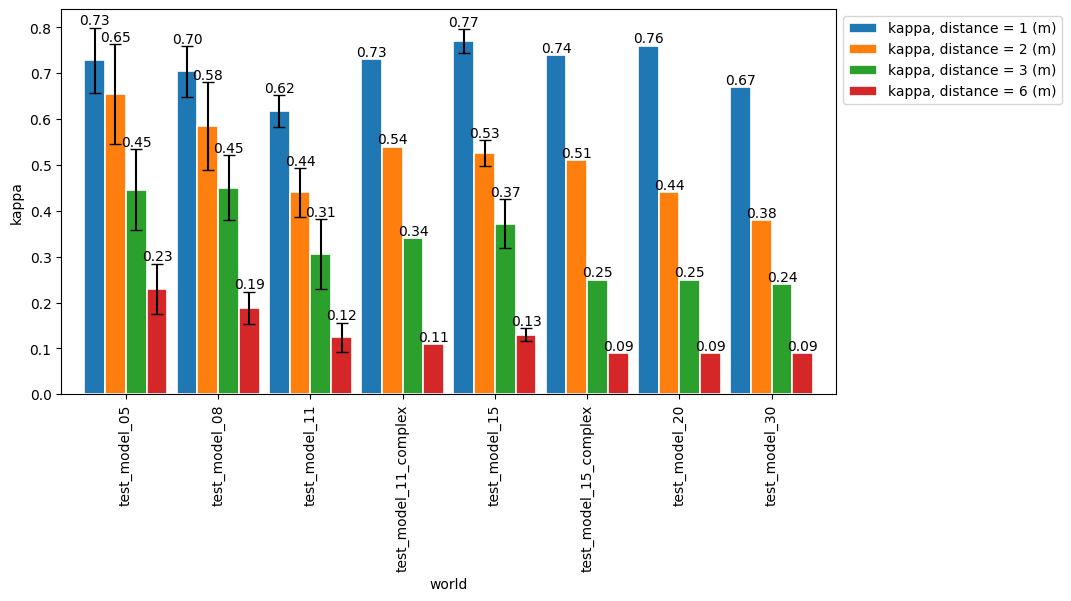
\includegraphics[width=\linewidth]{graphics/peinture_au_rouleau-kappa_vs_world_for_each_d.png}
		\caption{$\kappa$ according to the density of the world.}
		\label{fig:peinture_au_rouleau-kappa_vs_world}
	\end{subfigure}
	\hfill
	\begin{subfigure}[t]{0.9\linewidth}
			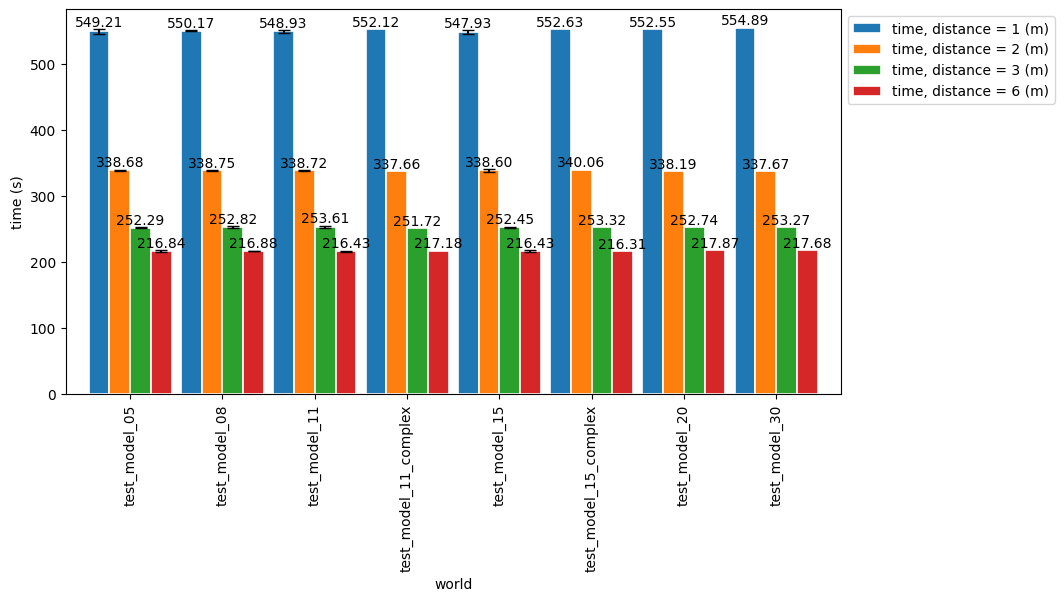
\includegraphics[width=\linewidth]{graphics/peinture_au_rouleau-time_vs_world_for_each_d.png}
			\caption{Runtime based on world density.}
			\label{fig:peinture_au_rouleau-time_vs_world}
	\end{subfigure}
	\caption{Evolution of Cohen's $\kappa$ and the execution time of the \textit{Roller Painting} algorithm as a function of the density of the world and the distance between the robots.}
	\label{fig:peinture_au_rouleau-world}
\end{figure}

First, we can observe that the Cohen score generally decreases with the number of corrosion zones.
There are exceptions, notably for the map composed of 15 corrosion zones, where the Cohen score is higher than for the maps composed of 5, 8 and 11 corrosion zones.
This is explained by the fact that in the maps composed of 5, 8 and 11 corrosion zones, we have introduced corrosion zones with elongated shapes unlike the map composed of 15 corrosion zones where the corrosion zones are all circles .
Indeed, elongated corrosion zones have a greater probability of causing phantom zones to appear, illustrated in figure~\ref{fig:ghost_zone}, than circular corrosion zones.
These phantom zones are areas free of corrosion which are detected by the crawlers.
These are therefore false positives which reduce the Cohen score.
These phantom zones are also more likely to appear when the density of the world is high and therefore the corrosion zones are closer to each other, or when the distance $d$ between the two crawlers is high.
This is what we can observe in figure~\ref{fig:peinture_au_rouleau-kappa_vs_distance} where the Cohen score decreases when the distance $d$ between the two crawlers increases.
We observe that there seems to be a linear relationship between the Cohen score and the distance $d$ between the two crawlers.

\begin{figure}[h!]
	\begin{subfigure}[t]{0.49\linewidth}
		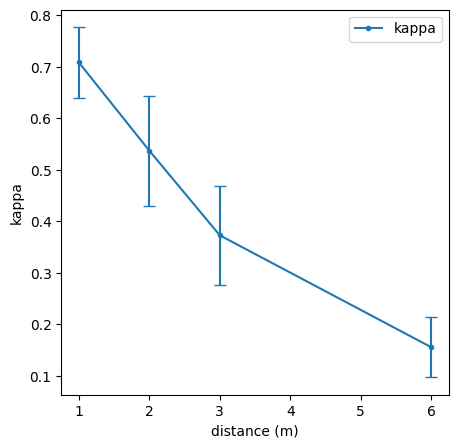
\includegraphics[width=\linewidth]{graphics/peinture_au_rouleau-kappa_vs_distance.png}
		\caption{$\kappa$ depending on the distance between the two crawlers.}
		\label{fig:peinture_au_rouleau-kappa_vs_distance}
	\end{subfigure}
	\hfill
	\begin{subfigure}[t]{0.49\linewidth}
			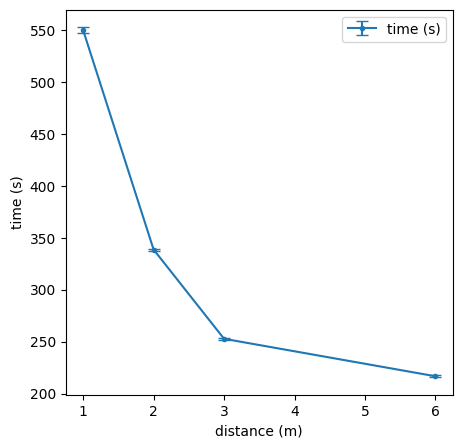
\includegraphics[width=\linewidth]{graphics/peinture_au_rouleau-time_vs_distance.png}
			\caption{Runtime depending on the distance between the two crawlers.}
			\label{fig:peinture_au_rouleau-time_vs_distance}
	\end{subfigure}
	\caption{Evolution of Cohen's $\kappa$ and the execution time of the \textit{Roller Painting} algorithm as a function of the distance between the two crawlers.}
	\label{fig:peinture_au_rouleau-distance}
\end{figure}

\begin{figure}[h!]
	\centering
	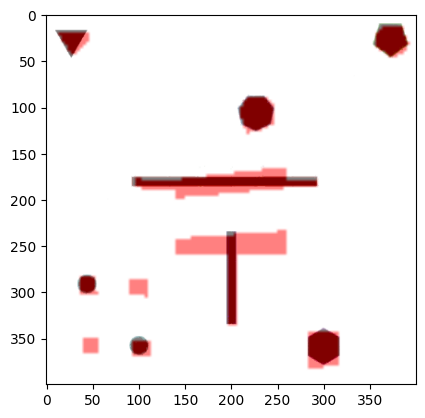
\includegraphics[width=0.5\linewidth]{graphics/output.png}
	\caption{Example of a phantom zone located at the bottom left of the map.}
	\label{fig:ghost_zone}
\end{figure}

Then, we observe that the execution time of the \textit{Roller Painting} algorithm is constant for each value of the number of corrosion zones.
This was expected because the algorithm in question is an \textit{a priori} algorithm and therefore does not depend on the number of corrosion zones.
On the other hand, the execution time depends on the distance $d$ between the two crawlers.
As we can see in figure~\ref{fig:peinture_au_rouleau-time_vs_distance}, the execution time increases when the distance $d$ between the two crawlers decreases.
This is because the greater the distance $d$, the fewer moves the crawlers have to make to cover the map.
There does not seem to be a linear relationship between the execution time and the distance $d$ between the two crawlers.
However, we would have expected that there would be a linear relationship between the execution time and the distance $d$ between the two crawlers.
It would be interesting to check if there was no bias introduced during the implementation of the algorithm.

We have also introduced two maps with more complex shapes than the base maps.
These are visible in the appendix~\ref{annexe:cartes}, in figures~\ref{fig:test_model_11_complex_1} and~\ref{fig:test_model_15_complex_1}.
Unfortunately, we could not, for the sake of time, vary the position of the corrosion zones, as we did with the low density maps.
However, there seems to be no significant difference between complex shaped maps and simple shaped maps.
For example, for the maps with 15 forms of corrosion and the map with 15 complex forms of corrosion, the Cohen score only varies by 0.02 on average for a distance $d = 1$ and by 0.04 on average for a distance $d = 6$.

In the rest of this report, we will consider a distance $d = 3$ meters between the two crawlers for the \textit{Roller Painting} algorithm.

\subsection*{\textit{Nordic Skiing} navigation strategy}

We are now going to analyze the results obtained for the \textit{Nordic Skiing} algorithm.
As for the \textit{Roller Painting} algorithm, we varied the density of the world and the distance $d$ between the two crawlers, but also the stride $s$ used between the two crawlers.
The figure~\ref{fig:ski_nordique-world_d} presents the evolution of the Cohen score and the execution time of the algorithm \textit{Nordic Skiing} as a function of the density of the world for different values of the distance $d$ between the two crawlers and a stride $s = 3$ meters.

\begin{figure}[h!]
	\centering
	\begin{subfigure}[t]{0.9\linewidth}
		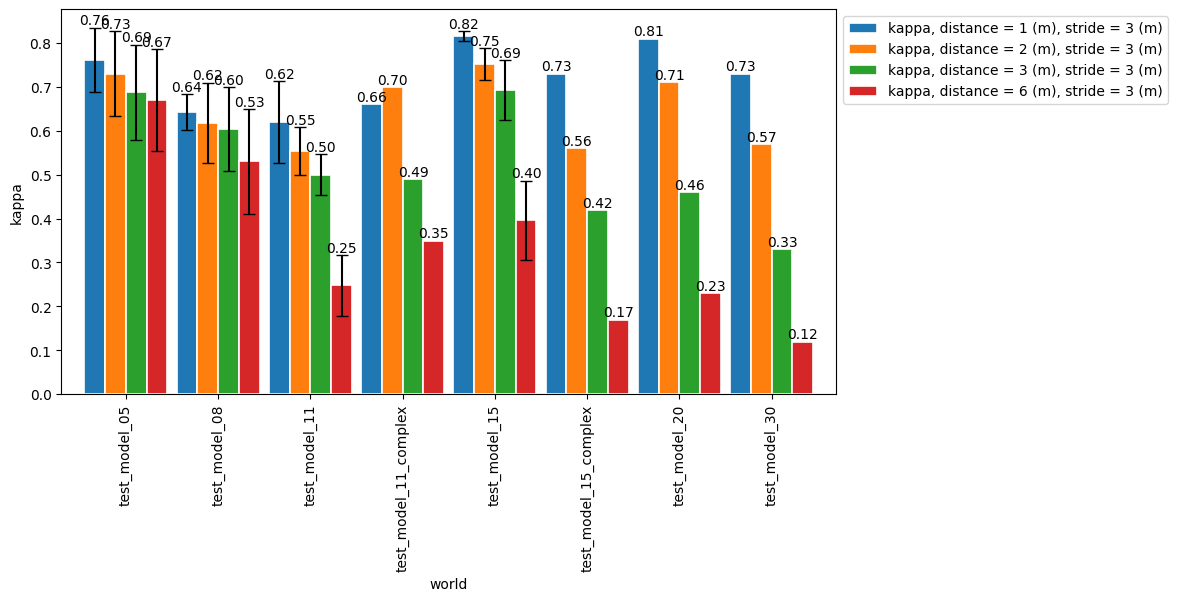
\includegraphics[width=\linewidth]{graphics/ski_nordique-kappa_vs_world_for_each_d.png}
		\caption{$\kappa$ according to the density of the world.}
		\label{fig:ski_nordique-kappa_vs_world_d}
	\end{subfigure}
	\hfill
	\begin{subfigure}[t]{0.9\linewidth}
		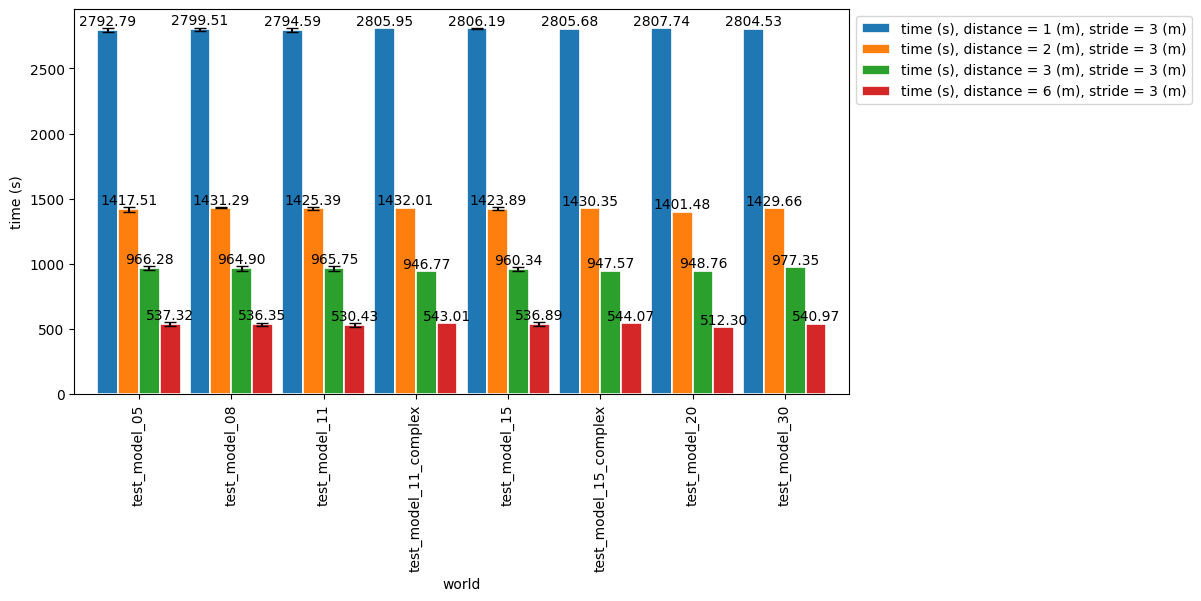
\includegraphics[width=\linewidth]{graphics/ski_nordique-time_vs_world_for_each_d.png}
		\caption{Runtime based on world density.}
		\label{fig:ski_nordique-time_vs_world_d}
	\end{subfigure}
	\caption{Evolution of Cohen's $\kappa$ and the execution time of the \textit{Nordic Skiing} algorithm as a function of the density of the world for different values of the distance between the two crawlers.}
	\label{fig:ski_nordique-world_d}
\end{figure}

We have very similar results to those obtained for the \textit{Roller Painting} algorithm.
Indeed, we observe in figure~\ref{fig:ski_nordique-kappa_vs_world_d} that the Cohen score generally decreases when the density of the world increases.
Moreover, the execution time of the algorithm \textit{Nordic Skiing}, observed in figure~\ref{fig:ski_nordique-time_vs_world_d}, is constant for each value of the density of the world.

\begin{figure}[h!]
	\centering
	\begin{subfigure}[t]{0.9\linewidth}
		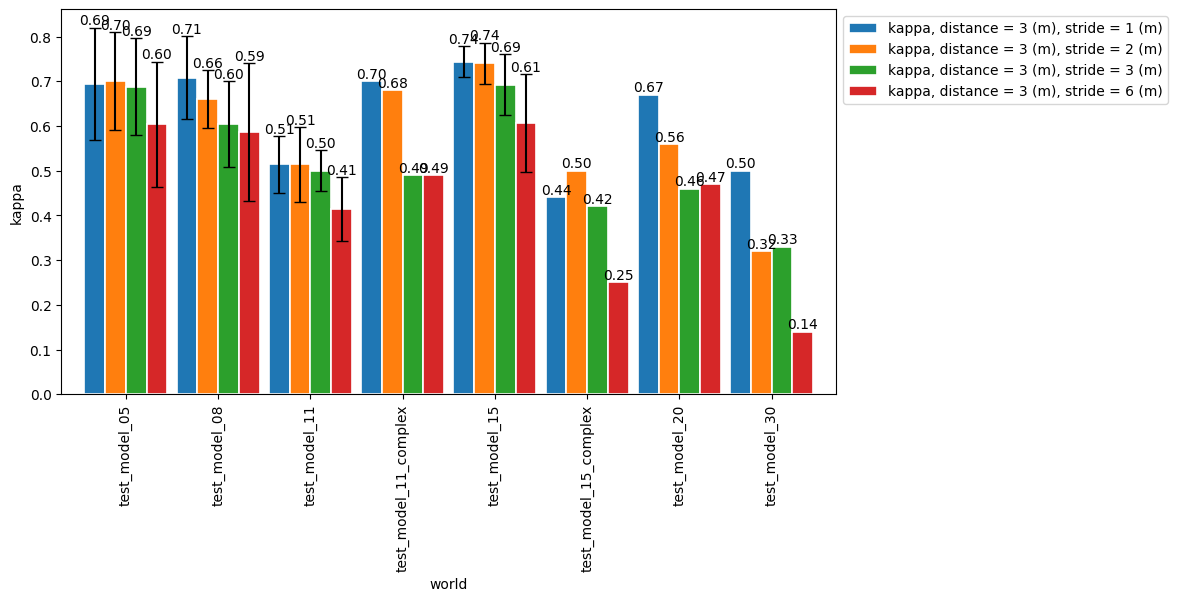
\includegraphics[width=\linewidth]{graphics/ski_nordique-kappa_vs_world_for_each_s.png}
		\caption{$\kappa$ according to the density of the world.}
		\label{fig:ski_nordique-kappa_vs_world_s}
	\end{subfigure}
	\hfill
	\begin{subfigure}[t]{0.9\linewidth}
		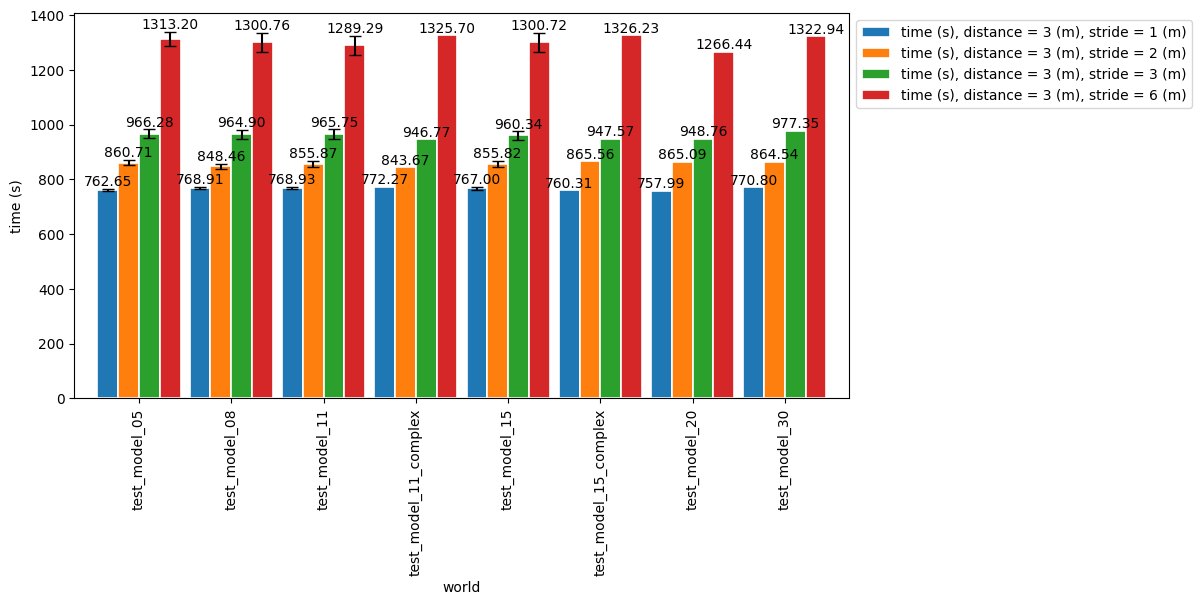
\includegraphics[width=\linewidth]{graphics/ski_nordique-time_vs_world_for_each_s.png}
		\caption{Runtime based on world density.}
		\label{fig:ski_nordique-time_vs_world_s}
	\end{subfigure}
	\caption{Evolution of Cohen's $\kappa$ and the execution time of the \textit{Nordic Skiing} algorithm according to the density of the world for different values of the stride between the two crawlers.}
	\label{fig:ski_nordique-world_s}
\end{figure}

We can observe in the figure~\ref{fig:ski_nordique-world_s} the evolution of the Cohen score and the execution time of the algorithm \textit{Nordic Skiing} according to the density of the world for different values of the stride $s$ between the two crawlers, and a distance $d = 3$ meters between the crawlers.
in the figure~\ref{fig:ski_nordique-kappa_vs_world_s}, we observe that the Cohen score is the lowest for large values of densities and large values of $d$, as for $d = 6$ meters and the maps with 30 and 20 corrosion areas.
This is explained by the fact that for large values of densities and $d$, the probability that the signal rays cross corrosion zones is higher.
There is therefore a greater chance that phantom zones will be created, which lowers Cohen's score.
The elongated shapes of the corrosion zones are also a factor that lowers the Cohen score as studied previously.
This is why we observe that the Cohen score is the highest for the map with the smallest density and without elongated forms of corrosion, that is to say the map with 15 corrosion zones.

In figure~\ref{fig:ski_nordique-time_vs_world_s}, we observe that the execution time of the algorithm \textit{Nordic Skiing} is constant for each value of the density of the world.
This was expected as for the \textit{Roller Painting} strategy.
However, we observe that the execution time varies with the stride $s$ used.
We would have rather expected the execution time to remain constant with the pitch of the crawlers.
Indeed, regardless of the value of the stride, the vertical and horizontal distance to be covered by the crawlers remains the same.
This significant difference in execution time is due to the way we implemented the \textit{Nordic Skiing} algorithm, which is not optimal.
We did not make the crawlers stop at the ends of the plates, but we made them continue by a value of the stride $s$, in addition, for simplicity of implementation, without thinking that the impact on the time of execution would be significant.

\begin{figure}[h!]
	\begin{subfigure}[t]{0.49\linewidth}
		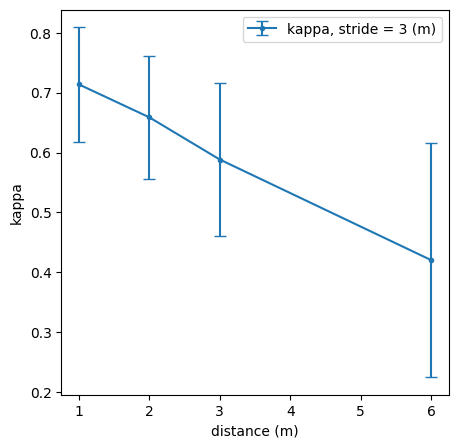
\includegraphics[width=\linewidth]{graphics/ski_nordique-kappa_vs_distance.png}
		\caption{$\kappa$ according to the distance between the two crawlers.}
		\label{fig:ski_nordique-kappa_vs_distance}
	\end{subfigure}
	\hfill
	\begin{subfigure}[t]{0.49\linewidth}
		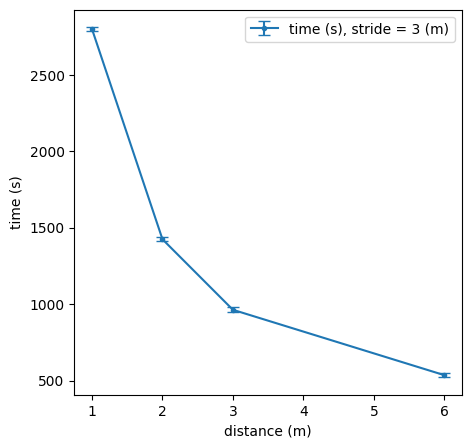
\includegraphics[width=\linewidth]{graphics/ski_nordique-time_vs_distance.png}
		\caption{Runtime according to the distance between the two crawlers.}
		\label{fig:ski_nordique-time_vs_distance}
	\end{subfigure}
	\caption{Evolution of Cohen's $\kappa$ and the execution time of the \textit{Nordic Skiing} algorithm according to the distance between the two crawlers.}
	\label{fig:ski_nordique-distance}
\end{figure}

In the figure~\ref{fig:ski_nordique-distance}, we observe the evolution of the Cohen score and the execution time of the algorithm \textit{Nordic Skiing} according to the distance which separates the two crawlers for a stride of 3 meters.
The score seems, as for the strategy \textit{Roller Painting}, to follow a linear relation with the distance which separates the two crawlers.
Execution time also appears to follow a linear relationship with the distance between the two crawlers.
The fact that the curve in figure~\ref{fig:ski_nordique-time_vs_distance} is not a straight line is due to the fact that the smaller the distance between the crawlers, the greater the number of rotations that the crawlers must perform.
However, the rotation time is not negligible in the execution times of the algorithms.

\begin{figure}[h!]
	\begin{subfigure}[t]{0.49\linewidth}
		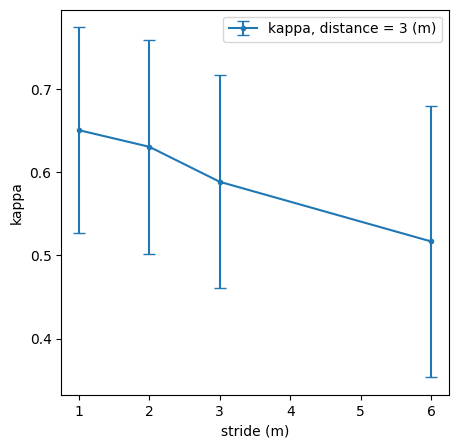
\includegraphics[width=\linewidth]{graphics/ski_nordique-kappa_vs_stride.png}
		\caption{$\kappa$ according to crawler stride.}
		\label{fig:ski_nordique-kappa_vs_stride}
	\end{subfigure}
	\hfill
	\begin{subfigure}[t]{0.49\linewidth}
		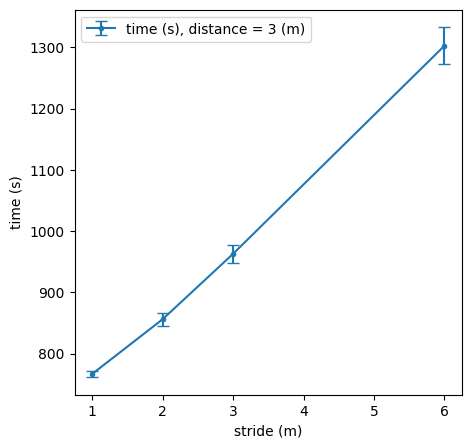
\includegraphics[width=\linewidth]{graphics/ski_nordique-time_vs_stride.png}
		\caption{Runtime according to crawler stride.}
		\label{fig:ski_nordique-time_vs_stride}
	\end{subfigure}
	\caption{Evolution of Cohen's $\kappa$ and the execution time of the \textit{Nordic Skiing} algorithm according to the crawler stride.}
	\label{fig:ski_nordique-stride}
\end{figure}

In the figure~\ref{fig:ski_nordique-stride}, we observe the evolution of the Cohen score and the execution time of the algorithm \textit{Nordic skiing} according to the crawlers' stride $s$ for a distance $d = 3$ meters.
The score seems to follow a linear relationship with the stride of the crawlers.
The smaller the stride, the higher the score.
This is consistent with what we explained previously.
The larger the stride, the greater the chance of creating phantom zones and therefore of reducing Cohen's score.
It should be noted however that there is a large variation in the score for the different values of the stride.
It therefore seems that the impact of the value of the stride on the score is rather weak unlike the impact of the value of the distance on the score.
Execution time seems to follow a linear relationship with crawler pace.
As explained previously, the latter should have been constant, but our implementation makes the execution time depend on the stride of the crawlers.

Again, it seems that the score and execution time are not affected by whether the shapes are complex or not.

In the rest of this report, we will consider a distance $d = 3$ between the two crawlers and a stride $s = 3$ for the algorithm \textit{Nordic Skiing}.

\subsection*{\textit{Polygonal Investigation} navigation strategy}

We then tested the \textit{Polygonal Investigation} algorithm on worlds composed of 5, 8 and 11 corrosion zones.
The inspection strategy is based on the results of the \textit{Roller Painting} strategy.
As explained previously, we justify this choice by the fact that the \textit{Roller Painting} strategy is the fastest of the \textit{a priori} strategies that we have implemented.

\begin{figure}[h!]
	\begin{subfigure}[t]{0.9\linewidth}
		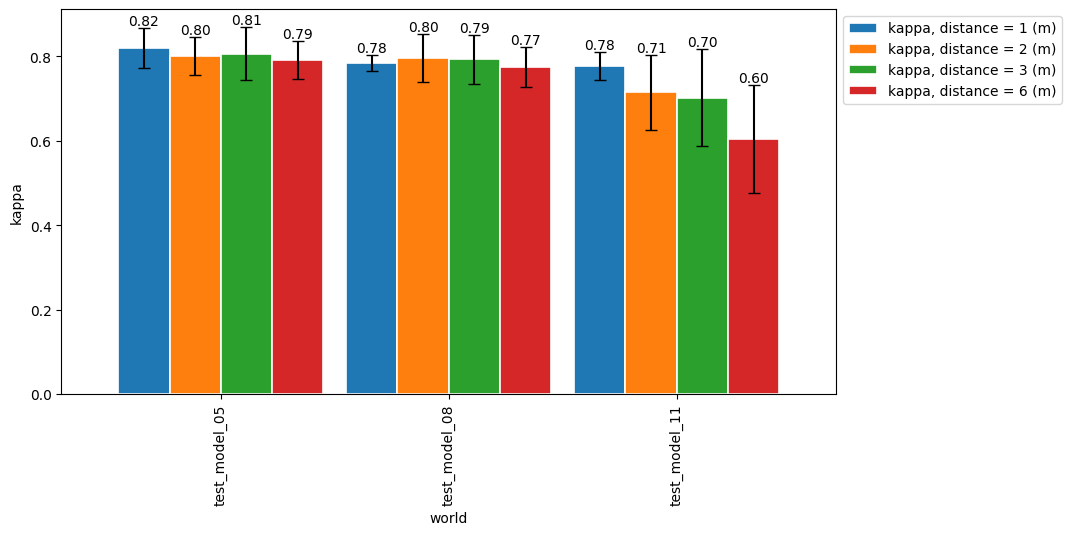
\includegraphics[width=\linewidth]{graphics/investigation_polygonale-kappa_vs_world_for_each_d_k1_n2_p4.png}
		\caption{$\kappa$ according to the density of the world.}
		\label{fig:investigation_polygonale-kappa_vs_world_for_each_d_k1_n2_p4}
	\end{subfigure}
	\hfill
	\begin{subfigure}[t]{0.9\linewidth}
		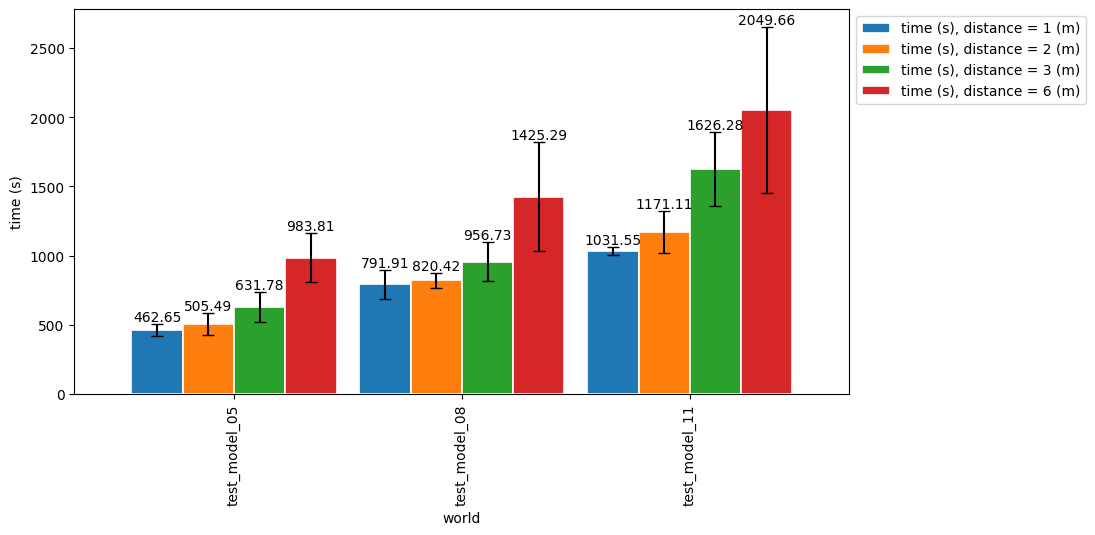
\includegraphics[width=\linewidth]{graphics/investigation_polygonale-time_vs_world_for_each_d_k1_n2_p4.png}
		\caption{Runtime based on world density.}
		\label{fig:investigation_polygonale-time_vs_world_for_each_d_k1_n2_p4}
	\end{subfigure}
	\caption{Evolution of Cohen's $\kappa$ and \textit{Polygonal Investigation} algorithm runtime according to the world density for different distances between crawlers with a 4-sided polygon.}
	\label{fig:investigation_polygonale-world_for_each_d_k1_n2_p4}
\end{figure}

The figure~\ref{fig:investigation_polygonale-kappa_vs_world_for_each_d_k1_n2_p4} shows the evolution of the Cohen score according to the density of the world for each value of $d$ used in the strategy \textit{Roller Painting}.
We used a 4-sided investigation polygon.
First, we observe Cohen scores relatively independent of distance between crawlers for maps with 5 and 8 corrosion zones.
This is an exciting result, because it means that we can use the \textit{Polygonal Investigation} strategy based on the results of the \textit{Roller Painting} strategy using a large distance between the crawlers, and therefore, a very fast \textit{Roller Painting} strategy.
Nevertheless, we can observe that for maps with 11 corrosion zones, the Cohen score is impacted by the distance between the crawlers, when the latter increases.
We attribute this result to the fact that this map has elongated corrosion zones very close to each other, having the effect of blocking certain rays emitted and received during the polygonal inspection of an area.
Polygonal inspection is therefore naturally impacted by the density of the world.
However, we can imagine, when repairing metal structures, that it is more convenient to merge corrosion areas close to each other into a single corrosion area, although this is not considered in our problem.

Figure~\ref{fig:investigation_polygonale-time_vs_world_for_each_d_k1_n2_p4} shows the evolution of execution time according to the world density for each value of $d$ used in the strategy \textit{Roller Painting}.
We used a 4-sided investigation polygon.
We observe that the execution time increases with the density of the world in a linear way.
This is an expected result, because the \textit{Polygonal Investigation} algorithm has linear complexity as a function of the number of corrosion zones, the latter consisting in traversing all the potential corrosion zones and inspecting them.
We also observe that the execution time increases with the distance between the crawlers.
Indeed, the greater the distance between the crawlers, the greater the number of phantom zones at the end of the \textit{Roller Painting} navigation strategy, and therefore the greater the number of potential corrosion zones.
However, these phantom areas are quickly processed by the \textit{Polygonal Investigation} algorithm.
For example, for map 5 with 11 corrosion areas, we get 12 potential corrosion areas with a distance of 1 meter between crawlers after the \textit{Roller Painting} strategy, versus 20 potential corrosion areas with a distance of 6 meters between the crawlers.
However, we observe an execution time of 1027 seconds for the first configuration versus 1616 seconds for the second configuration.
So we have for a 67\% increase in the number of potential corrosion areas, a 57\% increase in execution time.
The performance gain is not very large, but is still significant.

\begin{figure}[h!]
	\begin{subfigure}[t]{0.9\linewidth}
		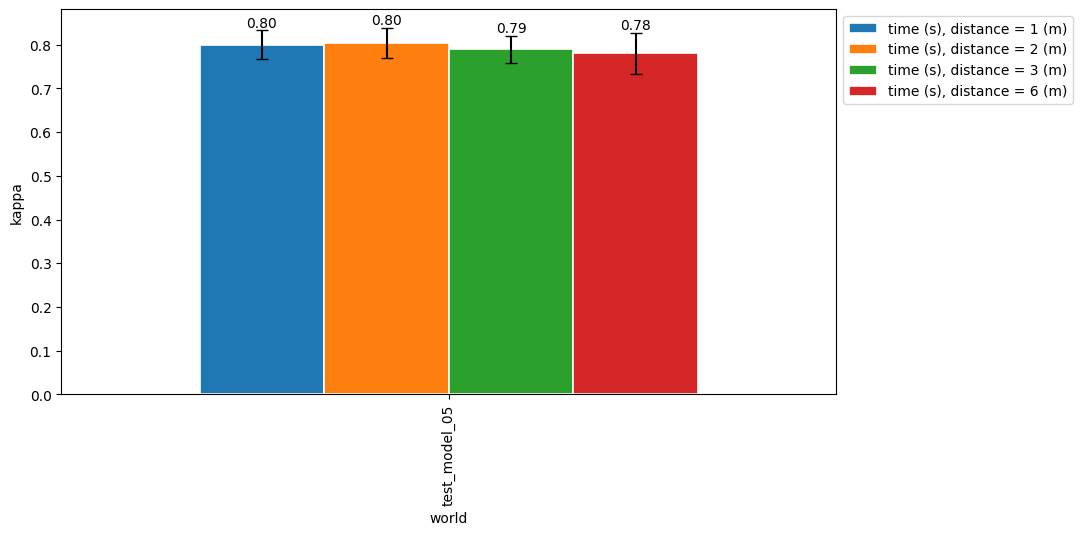
\includegraphics[width=\linewidth]{graphics/investigation_polygonale-kappa_vs_world_for_each_d_k1_n2_p6.png}
		\caption{$\kappa$ according to the density of the world.}
		\label{fig:investigation_polygonale-kappa_vs_world_for_each_d_k1_n2_p6}
	\end{subfigure}
	\hfill
	\begin{subfigure}[t]{0.9\linewidth}
			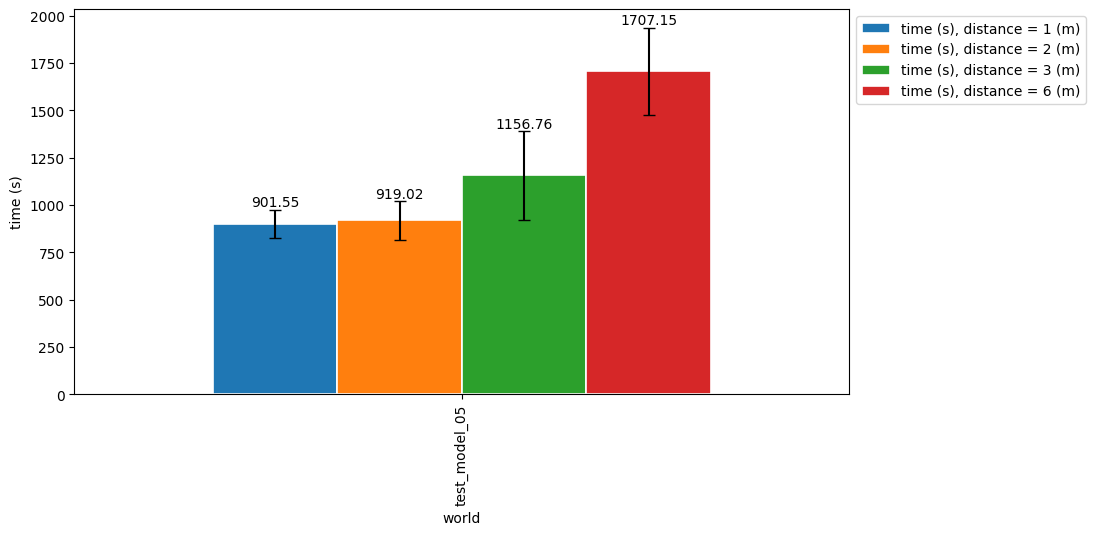
\includegraphics[width=\linewidth]{graphics/investigation_polygonale-time_vs_world_for_each_d_k1_n2_p6.png}
			\caption{Runtime based on world density.}
			\label{fig:investigation_polygonale-time_vs_world_for_each_d_k1_n2_p6}
	\end{subfigure}
	\caption{Evolution of Cohen's $\kappa$ and \textit{Polygonal Investigation} algorithm runtime according to the world density for different distances between crawlers with a 6-sided polygon.}
	\label{fig:investigation_polygonale-world_for_each_d_k1_n2_p6}
\end{figure}

We also varied the size of the investigation polygon of the \textit{Polygon Investigation} strategy.
We present in figure~\ref{fig:investigation_polygonale-kappa_vs_world_for_each_d_k1_n2_p6} the evolution of the Cohen score as a function of the density of the world for map 5, for a polygon with 6 vertices.
First, we do not observe a significant improvement in the Cohen score when the size of the investigation polygon increases.
On the contrary, we observe an average decrease, although very weak, of the score.
In theory, increasing the size of the investigation polygon should make it possible to better approach the convex hull of the corrosion zones, and therefore to obtain a better Cohen score.
However, we are limited in our implementation by the resolution used for the discretization of the map.
% Thus, it is probable that increasing the size of the investigation polygon eliminates cells from the occupancy grid (at the periphery of the corrosion zones) where corrosion is actually present, because it has there existed a ray which crossed this same cell.
However, for a more precise resolution, we should observe an improvement in the Cohen score.

We present in the figure~\ref{fig:investigation_polygonale-time_vs_world_for_each_d_k1_n2_p6} the evolution of the execution time according to the density of the world for map 5, for a polygon with 6 vertices.
Here, we naturally observe an increase in execution time when the size of the investigation polygon increases.

We would also have liked to vary the number of robots used for the polygonal investigation as well as the number of robot teams.
However, we did not have time to implement a solution for managing collisions between robots.
It would be interesting in future work to implement such a solution and to analyze the performance of the \textit{Polygonal Investigation} algorithm with these different parameters.
Indeed, the execution time of the \textit{Polygonal Investigation} algorithm should decrease when $k$ and $n$ increase.

In the next subsection, we will compare the performance of the \textit{Polygonal Investigation} algorithm with those of the \textit{Roller Painting} and \textit{Nordic Skiing} algorithms.
To do this, we will consider an investigation polygon, for the polygonal investigation, with $p = 4$ vertices.


		
\chapter{Discussion}

% text of this chapter goes here
		
\chapter{Conclusion}

% text of this chapter goes here

		
% The environment used here (theappendices) is a wrapper for the basic appendices environment which changes the appearance of the title page and the structure and appearance of the appendices in the table of contents and PDF bookmarks. The original functionality can be restored by simply removing the 'the' from the \begin{} and \end{} statements below.

\begin{theappendices}

\chapter{Experimental Equipment}
A telescope and a spectrometer were used to analyze the sun. Many other instruments were used.

\chapter{Data Processing}
Data was processed before being added to this document.

\end{theappendices}
		\makeBibliography
		% % Vita should only be included for PhD candidates.

\begin{vita}

Clark Kent was born on April 18, 1938, and adopted by parents Jonathan and Martha Kent in Kansas. He currently resides in the city of Metropolis, where his reporting for the Daily Planet has earned him critical acclaim both at home and abroad. He frequently collaborates with such fellow journalists as his Pulitzer-winning wife Lois Lane, close friend James ``Jimmy'' Olsen,  and longtime editor Perry White.

Clark and Lois enjoy their quiet time together, when they can play with their dog and their teenage son, Jonathan.

\end{vita}
	\end{thesisbody}

\end{document}
